
\documentclass[a4paper]{article}
\usepackage{fullpage} % Package to use full page
\usepackage{parskip} % Package to tweak paragraph skipping
\usepackage{tikz} % Package for drawing
\usepackage[light,math]{iwona}
\usepackage[T1]{fontenc}
\usepackage{amsmath, amssymb, amsthm}
\usepackage{amsfonts}
\usepackage{hyperref}
\usepackage{bbm}
\usepackage{mathabx}
\usepackage{url}
\usepackage{graphicx}
\usepackage{listings}
\usepackage{float}
\usepackage{tikz-cd}
\usepackage{mathtools}
\lstloadlanguages{[5.2]Mathematica}
\usepackage[pagewise]{lineno} %linenumbering
%\linenumbers %linenumbering
\usepackage{imakeidx}
\usepackage{stackrel}
\makeindex
\usepackage[a4paper,
bindingoffset=0in,
left=0.25in,
right=0.25in,
top=0.25in,
bottom=0.25in,
footskip=0.2in]{geometry}
\graphicspath{ {./images/} }
\usepackage[most]{tcolorbox}
\newtcolorbox{mytextbox}[1][]{%
	sharp corners,
	enhanced,
	colback=white,
	height=3cm,
	attach title to upper,
	#1
}
%\usepackage{coffee4} %coffeestain
%\setcounter{section}{-1}
\theoremstyle{plain}
\newtheorem{theorem}{Theorem}[section] % reset theorem numbering for each chapter
\newtheorem{corollary}[theorem]{Corollary}
\newtheorem{lemma}[theorem]{Lemma}
\newtheorem{prop} [theorem]{Proposition}
\theoremstyle{definition}
\newtheorem{defn}[theorem]{Definition}% definition numbers are dependent on theorem numbers
\newtheorem{eg}[theorem]{Example}
\newtheorem{rem}[theorem]{Remark}
\newtheorem{as}[theorem]{Assumption}
\newtheorem{ex} [theorem]{Exercise}
\newtheorem{example} [theorem]{Example}
\newtheorem*{proofqed}{\it{\textsl{Proof}}} %proof without the qed symbol

\newtheorem{notation}[theorem]{Notation}
\newtheorem*{claim*}{Claim}

\newcommand{\A}{\mathbb{A}}
\newcommand{\C}{\mathbb{C}}
\newcommand{\D}{\mathbb{D}}
\newcommand{\E}{\mathbb{E}}
\newcommand{\F}{\mathbb{F}}
\newcommand{\HH}{\mathbb{H}}
\newcommand{\I}{\mathbb{I}}
\newcommand{\K}{\mathbb{K}}
\newcommand{\PP}{\mathbb{P}}
\newcommand{\Q}{\mathbb{Q}}
\newcommand{\R}{\mathbb{R}}
\newcommand{\es}{\mathbb{S}}
\newcommand{\T}{\mathbb{T}}
\newcommand{\U}{\mathbb{U}}
\newcommand{\V}{\mathbb{V}}
\newcommand{\Z}{\mathbb{Z}}
\newcommand{\N}{\mathbb{N}}
\newcommand{\Ail}{\mathcal{A}}
\newcommand{\Bil}{\mathcal{B}}
\newcommand{\Cil}{\mathcal{C}}
\newcommand{\Eil}{\mathcal{E}}
\newcommand{\Fil}{\mathcal{F}}
\newcommand{\Gil}{\mathcal{G}}
\newcommand{\Hil}{\mathcal{H}}
\newcommand{\Iil}{\mathcal{I}}
\newcommand{\Lil}{\mathcal{L}}
\newcommand{\Mil}{\mathcal{M}}
\newcommand{\Nil}{\mathcal{N}}
\newcommand{\Oil}{\mathcal{O}}
\newcommand{\Pil}{\mathcal{P}}
\newcommand{\Qil}{\mathcal{Q}}
\newcommand{\Ril}{\mathcal{R}}
\newcommand{\Sil}{\mathcal{S}}
\newcommand{\Til}{\mathcal{T}}
\newcommand{\Uil}{\mathcal{U}}
\newcommand{\Vil}{\mathcal{V}}
\newcommand{\Xil}{\mathcal{X}}
\newcommand{\bff}{\boldsymbol{f}}
\newcommand{\bfx}{\boldsymbol{x}}
\newcommand{\bfy}{\boldsymbol{y}}
\newcommand{\bfz}{\boldsymbol{z}}
\newcommand{\brw}{\boldsymbol{\mathrm{w}}}
\newcommand{\Fnoise}{F_{\mathrm{noise}}}
\newcommand{\One}{\mathbbm{1}}
\newcommand{\xn}{\{ x_n \}_{n=1}^{\infty}}
\newcommand{\CB}{C_{\mathcal{B}}}
\newcommand\restr[2]{\ensuremath{\left.#1\right|_{#2}}}
\newcommand{\fkN}{\mathfrak{N}}
\newcommand{\crd}{\delta_{\mathrm{cr}}}
\newcommand{\hbeq}{\sim_{\mathrm{hb}}}
\newcommand{\qceq}{\sim_{\mathrm{qc}}}
\newcommand{\topeq}{\sim_{\mathrm{top}}}
\newcommand{\confeq}{\sim_{\mathrm{conf}}}
\newcommand{\hypdim}{\mathrm{HD}_{\mathrm{hyp}}}
\newcommand{\HD}{\mathrm{HD}}
\newcommand{\area}{\mathrm{area}}
\newcommand{\diam}{\mathrm{diam}}
\newcommand{\orb}{\mathrm{orb}}
\newcommand{\limn}{\lim\limits_{n\to+\infty}}
\newcommand{\limm}{\lim\limits_{m\to+\infty}}
\newcommand{\liml}{\lim\limits_{l\to+\infty}}
\newcommand{\limk}{\lim\limits_{k\to+\infty}}
\newcommand{\limi}{\lim\limits_{i\to+\infty}}
\newcommand{\limt}{\lim\limits_{t\to+\infty}}




\title{IFS2023 Reading Group Notes}
\author{ICMC-USP}
\date{2023}

\begin{document}

\maketitle

\tableofcontents

\section{The space where fractals live (09/03)}
Welcome to the first session of this series of meetings on Iterated Function Systems. This is such an interesting subject because it is a unified way of constructing fractals (containing classical Cantor sets, Sierpinski gaskets, the Barnsley fern, etc.) and also has quite nice applications, such as fractal image compressing.

Iterated function systems offer a new perspective for fractals, in opposition to the view that those sets resulted from successive microscopic refinement. We will now look at fractals as attractors of iterated function systems (a much more global perspective).

We'll start defining Iterated Function Systems as a complete metric space $M$ together with a collection of maps \textbf{f} on M, that is $\textbf{f} = \{f_i : i=1,...,k\} \textnormal{ where } f_i:M\rightarrow M$

\begin{figure}[H]
    \centering
    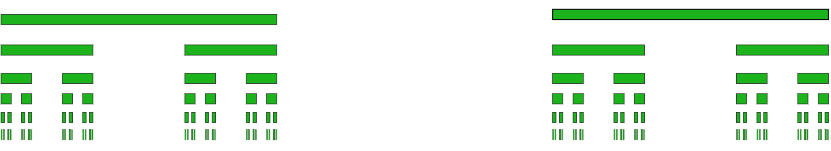
\includegraphics[scale=0.4]{img/cantor_ternary_set.png}
    \caption{The Cantor ternary set can be produced using an IFS}
    \label{fig:cantor_ternary}
\end{figure}

Let us in this first session concentrate on constructing some important definitions and theorems about the space we'll be working on.

Let (M,d) be a metric space and define
\begin{enumerate}
    \item For $a \in M$, $B \neq \emptyset$, $d_1(a,B) := inf_{b \in B} d(a,b)$
    \item For nonempty $A, B \subseteq M$, $d_2(A,B) := sup_{a \in A} d_1(a,B)$
    \item The Hausdorff distance $d_H(A,B) = max\{d_2(A,B),d_2(B,A)\}$
\end{enumerate}

Note that the need for $d_H$ comes from the necessity of symmetry for the distance function (given that $d_2$ is not symmetric).

Now we define the central piece of this session, which is the collection of all nonempty compact subsets of M, denoted by $H(M)$ (called the space where fractals live).

\begin{prop}
$d_H$ a distance in $H(M)$.
\end{prop}
\textit{Proof}: 
\begin{enumerate}
    \item Symmetry: $max\{d_2(A,B),d_2(B,A)\} = max\{d_2(B,A),d_2(A,B)\}$.
    \item $d_H(A,B) < \infty$
    \item Non-negativity is immediate from definition (d is a distance).
    \item If $A=B$ then $d_H(A,B) = 0$: $d_H(A,B) = d_2(A,A) = sup_{a \in A} d_1(a,A) = sup_{a \in A} inf_{b \in A} d(a,b) = 0$.
    \item If $d_H(A,B) = 0$ then $A=B$: $d_2(A,B) = 0 = d_2(B,A) \therefore d_1(a,B) = 0 \forall a \in A \therefore A \subseteq B$ (similarly we prove $B \subseteq A$).
    \item Triangle inequality:
    
    With A, B and C compact sets we write
    \begin{align*}
        d_1(a, C) &= min_{c \in C} d(a,c) \leq min_{c \in C}[d(a,b) + d(b,c)] \textnormal{ for any } b \in B\\
        &= d(a,b) + min_{c \in C}(b,c) \textnormal{ for any } b \in B\\
        d_1(a,C) &\leq min_{b\in B}d(a,b) + min_{b \in B} min_{c \in C} d(b,c)\\
        &\leq min_{b \in B}d(a,b) + max_{b \in B} min_{c \in C} d(b,c)\\
        &=d_1(a,B) + d_2(B,C) \\
        \therefore d_2(A,C) &\leq d_2(C,B) + d_2(B,A)
    \end{align*}
    Now
    \begin{align*}
        d_H(A,C) &= max\{d_2(A,C), d_2(C,A)\}\\
        &\leq max\{d_2(A,B) + d_2(B,C), d_2(C,B) + d_2(B,A)\}\\
        &\leq max\{d_2(A,B),d_2(B,A)\} + max\{d_2(B,C),d_2(C,B)\} \\
        &= d_H(A,B) + d_H(B,C)
    \end{align*}
    \qedsymbol
\end{enumerate}

\section{The Hutchinson Operator (16/03)}
Let us focus on contraction mappings on the space of fractals previously established. We specify $f_1,...,f_k: M\rightarrow M$ being contractions with factors $\lambda_1, ..., \lambda_k$
$$\forall x,y \in M: d(f_i(x),f_i(y)) \leq \lambda_i d(x,y)$$
Also, denote $\lambda = max\{\lambda_1,...\lambda_k\}$.
\begin{defn}
    The Barnsley-Hutchinson operator $B:H(M) \rightarrow H(M)$ is given by
    $$B(A) = \cup^k_{i=1}f_i(A) \textnormal{ for all } A \in H(M)$$
\end{defn}

We'll be initially interested in four theorems regarding the Hutchinson operator, but before stating and proving them, we'll look at three interesting lemmas

\begin{lemma}
Let $f:M\rightarrow M$ be a contraction mapping on the metric space $(M,d)$. Then $f$ is continuous.
\end{lemma}
\textit{Proof:}

Let $\epsilon > 0$ be given. Let $\lambda > 0$ be the contraction factor for $f$. Then
$$d(f(x),f(y)) \leq \lambda d(x,y) < \epsilon$$
whenever $d(x,y) < \delta \textnormal{ with } \delta=\frac{\epsilon}{\lambda}$. \\ \qedsymbol

\begin{lemma}
    Let $f:M\rightarrow M$ be a continuous mapping on the metric space $(M,d)$. Then $f$ maps $H(M)$ into itself.
\end{lemma}

\textit{Proof:}

Let S be a nonempty compact subset of M. Then clearly $f(S) = \{f(x): x \in M\}$ is nonempty.

We want to show that $f(S)$ is compact. Let $\{y_n = f(x_n)\}$ be an infinite sequence of points in S. Then $\{x_n\}$ is an infinite sequence of points in S. Since S is compact there is a subsequence $\{x_{N}\}$ that converges to a point $\hat{x} \in S$.

But as $f$ is continuous it implies that $\{y_{N} = f(x_N)\}$ is a subsequence of $\{y_n\}$ that converges to $\hat{y} = f(\hat{x}) \in f(S)$.\\ \qedsymbol

\begin{lemma}
    Let $f:M\rightarrow M$ be a contraction mapping on the metric space $(M,d)$ with contraction factor $\lambda$. Then $f:H(M)\rightarrow H(M)$ defined by
    $$f(B) = \{f(x): x \in B\} \forall B \in H(M)$$
    is a contraction mapping on $(H(M),d_H)$ with contraction factor $\lambda$.
\end{lemma}

\textit{Proof:}

From lemma 2.1 $f:M\rightarrow M$ is continuous and from lemma 2.2 $f$ maps $H(M)$ into itself.

Now let $B, C \in H(M)$, then
\begin{align*}
    d_2(f(B),f(C)) &= max\{min\{d(f(x),f(y)): y \in C\}: x \in B\}\\
    &\leq max\{min\{\lambda d(x,y):y\in C\}:x \in B\} = \lambda d_2(B,C)
\end{align*}

Similarly $d_2(f(C),f(B)) \leq \lambda d_2(C,B)$. 

Finally, we write
$$d_H(f(B),f(C)) = max\{d_2(f(B),f(C)),d_2(f(C),f(B))\} \leq \lambda max\{d_2(B,C),d_2(C,B)\} \leq \lambda d_H(B,C)$$ \\ \qedsymbol



After the above lemmas, let's now look at four theorems regarding the Hutchinson Operator over the space of fractals.

\begin{theorem}
The operator B is a contraction in $(H(M),d_H)$ with factor $\lambda$.
\end{theorem}

We first prove the following proposition
\begin{prop}
If $A_1, ..., A_k, B_1, ..., B_k \in H(M)$, then $d_H(\cup A_i,\cup B_i) \leq max_i d_H(A_i,B_i)$
\end{prop}

\textit{Proof: }

If $C \in H(M)$, then
$$d_2(\cup A_i, C) = max_{x \in \cup A_i} d_1(x, C) = max_{i}max_{x \in A_i}d_1(x,C) = max_{i}d_2(A_i,C)$$
Which yields
$$d_2(\cup A_i,\cup B_i) = max_i d_2(A_i, \cup B_i) \leq max_i d_2(A_i,B_i)$$

Where last inequality is true because $d_2(A_i,\cup B_i) \leq d_2(A_i,B_i)$ for each $i$. In analogous way, we can prove $d_2(\cup B_i, \cup A_i) \leq max_i d_2(B_i,A_i)$.

Finally
\begin{align*}
    d_H(\cup A_i, \cup B_i) &= max\{d_2(\cup A_i, \cup B_i), d_2(\cup B_i, \cup A_i)\}\\
    &\leq max\{max_i d_2(A_i,B_i), max_i d_2(B_i,A_i)\}\\
    &\leq max_i d_H(A_i,B_i)
\end{align*}
\qedsymbol

\section{Contraction mappings on $H(M)$ and fixed point dependence on parameters (23/03)}

We start by proving Theorem 2.5

\textit{Proof of Theorem 1: }

For $K_1, K_2 \in H(M)$, we have

\begin{align*}
    d_H(B(K_1), B(K_2)) &= d_H(\cup_i f_i(K_1),\cup_i f_i(K_2))\\
    &\leq max_i d_H(f_i(K_1),f_i(K_2))\\
    &\leq max_i \lambda _i d_H(K_1,K_2) \leq \lambda d_H(K_1,K_2)
\end{align*}
\qedsymbol

\begin{theorem}
Let (M,d) be a complete metric space, and let $f: M\rightarrow M$ be a contraction with factor $\lambda$. Then, there is a unique point $p \in M$ such that $f(p) = p$. Moreover, p is an attracting fixed point (i.e., for any $y \in M$, the sequence $f^n(y)$ converges to p.)
\end{theorem}

\textit{Proof: }

Let $x \in M$, and consider the sequence $f^n(x) \in M$. For any $n \in \mathbf{N}$, we have
\begin{align*}
    d(x, f^n(x)) &\leq d(x, f^1(x)) + d(f^1(x), f^2(x)) + ... + d(f^{n-1}(x),f^n(x))\\
    &<d(x,f^1(x))(1 + \lambda + ... + \lambda^{n-1}) \\
    &< d(x, f^1(x))\Sigma^\infty_{n=0}\lambda^n < \infty
\end{align*}
Fixing $\epsilon > 0$ and choosing an integer N such that $\lambda^N d(x, f^1(x))\Sigma^{\infty}_{n=0}\lambda^n < \epsilon$. Then, for any $m \geq n \geq N$, we have
$$d(f^m(x),f^n(x)) = d(f^n\circ f^{m-n},f^n(x)) \leq \lambda^n d(f^{m-n}(x),x) \leq \lambda^N d(x,f^1(x))\Sigma^\infty_{n=0}\lambda^n < \epsilon$$

This shows that $f^n(x)$ is indeed a Cauchy sequence in M. But since $(M,d)$ is complete, $f^n(x)$ converges to some point $p$ in $M$.

Also, $p$ is a fixed point of $f$
$$f(p) = f(\lim_{n\rightarrow\infty}f^n(x)) = \lim_{n\rightarrow\infty}f\circ f^n(x) = \lim_{n\rightarrow\infty}f^{n+1}(x) = \lim_{n\rightarrow\infty}f^n(x) = p$$

To prove uniqueness, consider $q \in M$ also a fixed point of $f$. Then
$$d(p,q) = d(f(p),f(q)) \leq \lambda d(p,q) \therefore d(p,q) = 0 \textnormal{ and } p=q$$

Finally, taking any $y \in M$
$$d(f^n(y),p) = d(f^n(y),f^n(p)) \leq \lambda^n d(y,p) \rightarrow 0$$

Which yields $f^n(y) \rightarrow p$.

\qedsymbol

The next theorem follows immediately from our previous results.

\begin{theorem}
    (Collage) If $(M,d)$ is complete, then the Hutchinson operator $B$ has a unique fixed point $K \in H(M)$. It is attractive and it is called Hutchinson attractor.
\end{theorem}

Finally, we conclude this session with a view on the dependence of fixed points on the parameters of the contraction maps.
\begin{theorem}
    Let $(\Lambda, \rho)$ be a metric space and $(M,d)$ a complete metric space and let
    $$ T : \Lambda \times M \rightarrow M$$
    be a family of contractions with uniform contraction factor, that is
    $$d(T(\lambda,x), T(\lambda,y) ) \le k d (x,y) \mbox{,     } \forall \lambda \in \Lambda \mbox{   e  } \forall x,y \in M$$
    Suppose that for $x\in M$ the map $\lambda \mapsto T(\lambda, x)$ is continuous from $\Lambda$ to $M$. Then for each $\lambda \in \Lambda$, $T(\lambda, \cdot)$ has a unique fixed point $x(\lambda)$ and the map $\lambda \mapsto x(\lambda)$ is continuous.
\end{theorem}

\textit{Proof: }

Given $\lambda\in\Lambda$, take $x\in M$ such that
$$T(\lambda, x) = x = x(\lambda)$$

The existence of $x$ comes from the fact that $T$ is a contraction for a fixed $\lambda$.

From the hypothesis, for a fixed $\varepsilon_0>0$ there is a $\delta>0$ such that $\beta\in\Lambda$ with $\rho(\beta,\lambda) \le \delta$ implies in

$$d(T(\lambda,x),T(\beta,x) \le \varepsilon_0$$

Consider then $\beta\in \Lambda$ in the neighborhood of $\lambda $ and take $y\in M$ such that 
$$T(\beta, y) = y = y(\beta)$$

We can then write

$$d(x(\lambda),y(\beta)) = d(T(\lambda, x(\lambda)), T(\beta, y(\beta))$$
$$\le \underbrace{d(T(\lambda, x(\lambda)), T(\lambda, y(\beta))}_{k d(y(\beta),y(\beta)} +\underbrace{d(T(\lambda, y(\beta)), T(\beta, y(\beta))}_{\le \varepsilon_0} 
$$

Which yields

$$
d(x(\lambda),y(\beta)) \le \frac{\varepsilon_0}{1 - k}
$$

Therefore, $\forall \varepsilon>0$, taking $\delta>0$ such that $\varepsilon_0  = \varepsilon(1-k)$, we have

$$\rho(\lambda,\beta) \le \delta \Rightarrow d(x(\lambda),y(\beta)) \le \varepsilon$$

\qedsymbol

To visualize the highlighted dependence, we head to \textbf{https://ifs-fractals.herokuapp.com/playground} for some examples.

\section{Seminar Day 30/03/2023} 
 \subsection{Motivations} 
 \begin{itemize} 
   \item Review Topology; 
   \item Construct the $\sigma$-algebra that will be used; 
   \item Construct the Middle-Third Cantor set via sequences of functions randomly picked. 
 \end{itemize} 
  
 \subsection{The Usual Construction of the Cantor Set} 
 \subsubsection{Goal of the Part} 
  \paragraph{} Construction of the Cantor Set via nested intervals, analytical properties of the set, its topological properties and construction 
 via functions. 
 \subsubsection{Main Text} 
   Before getting on the construction forementioned, it's important to know how it's usually done, even if just a bit.  
 For that, we consider the interval $[0, 1].$ From it, we will delete the open middle third interval, i.e., $\biggl(\frac{1}{3}, \frac{2}{3}\biggr)$ 
 which will leave us with two line segments, namely $\biggl[0, \frac{1}{3}\biggr]\cup\biggl[\frac{2}{3}, 1\biggr] = C_{1}.$ Now, 
 repeat that for eacho one of these intervals and remove their open middle-third intervals, yielding  
 \begin{align*} 
   &\biggl[0, \frac{1}{9}\biggr],\quad\biggl[\frac{2}{9}, \frac{1}{3}\biggr]\\ 
   &\biggl[\frac{2}{3}, \frac{7}{9}\biggr],\quad \biggl[\frac{8}{9}, 1\biggr]. 
 \end{align*} 
   Then, we call their union $C_{2} = \biggl[0, \frac{1}{9}\biggr]\cup\biggl[\frac{2}{9}, \frac{1}{3}\biggr]\cup\biggl[\frac{2}{3}, \frac{7}{9}\biggr]\cup\biggl[\frac{8}{9}, 1\biggr].$ 
 We thus define inductively $C_{n}\coloneqq\displaystyle \frac{C_{n-1}}{3}\cup\biggl(\frac{2}{3}+\frac{C_{n-1}}{3}\biggr)$, and  
 define the middle-third Cantor set by  
   $$ 
   \boxed{\mathcal{C}\coloneqq \lim_{n\to\infty}C_{n} = \bigcap_{n=0}^{\infty}C_{n}} 
   $$ 
  
   Briefly speaking about this set's properties, it has the same cardinality as the real line. To prove it, we use Bernstein-Schr\oe der 
 theorem and compare the cardinality of $\mathcal{C}$ with that of $[0, 1].$ Thus, $\aleph_{1}\geq{|\mathcal{C}|}$ since $\mathcal{C}\subsetneq{[0, 1]}$. 
 On the other hand, to show the other side of the inequality, one constructs a surjection going from $\mathcal{C}$ to $[0, 1]$. 
 Jumping right to the definition, it is motivated by writing the points of the interval $[0, 1]$ in terms of base 3, and then removing 
 on each n step, the numbers that have 1 as their nth digit in the ternary representation. 
  
   On the first step, digits of the form $0.1aaaaaaaaaa\cdots$, where $aaaaaaaaa \cdots$ is between $00000\cdots_{3}$, and $22222 \cdots_{3}.$ 
 leaving only the numbers whose first digit is either 0 or 2. The next step removes numbers with 1 on the second coordinate, leaving only those 
 that assume the form $0.00aaaaa \cdots,0.02aaaaa \cdots, \text{ or } 0.22aaaaa\cdots$. We repeat it ad infinitum, and the numbers 
 remaining on the Cantor set haver representations consisting entirely of 0's and 2's. 
  
 Hence, the function from $\mathcal{C}$ to $[0, 1]$ takes the ternary numerals constructed above and replaces every 2's by 1's, in a way 
 that we interpret the sequence obtained as a binary form of a real number in $[0, 1]$, and reciprocally, any of them have a binary  
 representation that can be translated to a ternary representation of a number in the Cantor set by replacing 1's by 2's:  
   $$ 
   f\biggl(\sum\limits_{k\in \mathbb{N}}^{}a_{k}3^{-k}\biggr) = \sum\limits_{k\in \mathbb{N}}^{}\frac{a_{k}}{2}2^{-k},\quad \forall k\in \mathbb{N}: a_{k}\in \{0, 2\} 
   $$ 
   Therefore, f is surjective, so that $\aleph_{1} \leq{|\mathcal{C}|} \leq{\aleph_{1}.}$ 
  
   Some other interesting properties is that it is a set of measure 0, i.e., it is infinitesimally small, even though it has uncountably many 
 elements. It is self-similar, a sort of primitive fractals, because it is equal to two copies of itself when translated and dilated by some factor.  
 More specifically, dilating each copy by a factor of $\frac{1}{3}$ and translating it, and as a consequence, when you zoom in into a  
 part of the set, it looks identical to the whole. This can be seen from the equation given before, i.e.,  
   $$ 
     C_{n}\coloneqq\displaystyle \frac{C_{n-1}}{3}\cup\biggl(\frac{2}{3}+\frac{C_{n-1}}{3}\biggr), 
   $$ 
   and from here, the self-similarity follow by showing that $C\displaystyle \frac{C}{3}\cup\biggl(\frac{2}{3}+\frac{C}{3}\biggr)$. 
 The Cantor set is also perfect, meaning that any point in the Cantor Set has an infinite sequence of points also in the set converging to that point. 
 The proof of this statement relies on taking an element x in $\mathcal{C}$, and arbitrary $\epsilon > 0$, an $N(\epsilon)\in \mathbb{N}$ and finding a good enough M  
 so that $x\in[M, M+1]\subseteq{(x-\epsilon, x+\epsilon)}$. Then, we apply the process used on the construction of $\mathcal{C}$ to 
 the interval $[M, M+1]$, removing the interval $(\frac{3M+1}{3}, \frac{3M+2}{3})$ from it, to see that if were to belong to the removed  
 interval or not, it'd be a limit point in both cases. From arbitrariness of the choices, it follow that $\mathcal{C}$ is indeed a perfect set. 
  
   Topologically speaking, the Cantor set has nice properties too. It's totally disconnected, compact, perfect, nonempty, and metrizable. 
 Furthermore, any set with those properties are the Cantor Set up to homeomorphism. 
 \subsection{The Motivation Problem} 
 \subsubsection{Goal of the Part} 
  \paragraph{} Review the Hutchinson Attractor, give the motivation problem behind construction the Cantor Set as a random application of functions 
 that converge to the Attractor, set up the main problems to be studied. 
 \subsubsection{Main Text} 
   As Kevin talked about last week, we can construct the Cantor Middle-Third set through a function known as the Hutchinson Attractor, denoted by B, ranging 
 from the set $\mathcal{H}(M)$ of nonempty compact subsets of a metric space M to $\mathcal{H}(M)$ itself and given by the union of the images of  
 contractions in M. The way we construct it is, for instance, by applying B to a singleton set A = $\{x\}$ and using de previously defined metric $d_{H}$ to translate 
 the result to the Cantor Set. For each n iterations, we get an ammount of parts of the CMT set equal to $2^{n}.$  
 Now consider two functions $f_{i}:[0,1]\rightarrow [0, 1]$ 
   $$ 
     f_{i} = \left\{\begin{array}{ll} 
         \frac{x}{3}, \quad i=0\\ 
         \frac{x}{3}+\frac{2}{3}, \quad i=1\\ 
       \end{array}\right. 
   $$ 
   The infinite application of these functions yield the Cantor set, which shall be denoted by $\mathcal{C}$ to make things easier. In other words, 
 Consider now a representation of infinitely many combinations of 0's and 1's in any order, i.e., $\omega = (0, 1, 0, 0, 1, \cdots)$ and 
 let $f_{\omega}^{n}$ be the repeated use of $f_{i}$ as defined before using the indices from $\omega$, so that 
   $$ 
   f_{\omega}^{n}(x) = f_{\omega_{n-1}}\circ{\cdots}\circ{f_{\omega_{1}}}\circ{f_{\omega_{0}}}(x) 
   $$ 
   indicates that we start using the n-th coordinate of $\omega$ on each f. Using the example of $\omega$ from before, $f_{\omega}^{n}$ 
   would be 
   $$ 
     f_{\omega}^{n}(x) = f_{\omega_{n-1}}\circ{\cdots}\circ{f_{0}}\circ{f_{1}}\circ{f_{0}}(x). 
   $$ 
   Using that notation, the thesis given at the start that the infinite use of $f_{i}$ eventually covers all of $\mathcal{C}$ is the same as 
   $$ 
   \lim_{l\to\infty}\overline{\{f_{\omega}^{n}(x):n\geq{l}\}} = B 
   $$ 
   That begs the question: Will EVERY sequence of digits $\omega\in\{0, 1\}^{\mathbb{N}}$, when combined with $f_{i}$, give  
 as its image the Cantor set? In fact, the answer is no, as the theorem is stated 
  \begin{theorem}
    Let $\phi$ be an independent and identically distributed random product of contractions $f_{1},\cdots, f_{k}:M\rightarrow M$ and 
   K be the corresponding Hutchinson Attractor. Given $p\in M$, we have 
     $$ 
     \lim_{l\to\infty}\overline{\{f_{\omega}^{n}:n\geq{l}\}} = K 
     $$ 
     for $\mathbb{P}-$almost all $\omega.$ 
  \end{theorem} 
 On that note, to grasp what we mean by almost all sequences work, consider a sequence of a single digit, i.e., $\omega =\{0, 0, 0, \cdots\} $. Then, when we apply this to $f_{i}$, we get 
   \begin{align*} 
     f_{\omega}^{n}(x) &= f_{0}\circ{\cdots}f_{0}\circ{f_{0}}\circ{f_{0}}(x)\\ 
                       &= f_{0}\circ{\cdots}f_{0}(\frac{x}{3}) \\ 
                       &= f_{0}\circ{\cdots}f_{0}(\frac{x}{9}) \\ 
                       &\vdots\\ 
                       &= \frac{x}{3^{n}}. 
   \end{align*} 
   Because of this, as n goes to infinity, $f_{\omega}^{n}$ tends to 0, which is not the Cantor set. In other words, 
   $$ 
     \lim_{l\to\infty}\overline{\{f_{\omega}^{n}(x):n\geq{l}\}}\neq B. 
   $$ 
   a new problem arises, that is, will the number of $\omega$'s for which the initial thesis hold be way too small to be relevant? The answer is going to need 
 quite a bit of measure theory, for the answer is, in fact, that the result holds for almost every $\omega$. 
  
 \subsection{The Meaning of ``Almost Every''} 
   \subsubsection{Goals of this Part} 
   \paragraph{} We want to define $\sigma-algebras$, the foundation of what is a measure. Then, define measures properly speaking, what is a property that 
 happens almost everywhere, and some probabilistc concepts, such as independence and identical distributions. 
   \subsubsection{Main Text} 
   Now that the goal has been set, we can start to develop the theory needed to fully grasp it. Starting with a review of $\sigma-$algebra, 
 they are the sets in which we define measures. They are sets that have closure under countable unions and complements. Formally speaking,  
    
\textbf{Definition:}    Given a set $\Omega$, a $\sigma-$algebra $\mathcal{F}$ is a nonempty collection of subsets of $\Omega$ that satisfy 
   \begin{align*} 
     &(i) \text{ If }A\in \mathcal{F} \Rightarrow A^{c}\in \mathcal{F};\\ 
     &(ii) \text{ If } A_{i} \text{ is a countable sequence of sets, then } \bigcup_{i}A_{i}\in \mathcal{F};\\ 
     &(iii) \Omega\in \mathcal{F}.\square 
   \end{align*} 

  
  They are the defining ground that allow us to define measures and thus, find the meaning of ``Almost Every''. Without further ado, 
 we define a measure. 
\textbf{Definition:}    A measure is a nonnegative countably additive set function, i.e., a function $\mu:\mathcal{F}\rightarrow \mathbb{R}$ which satisfies 
   \begin{itemize} 
     \item[i)] $\mu(A)\geq{\mu(\emptyset)}=0$ for all $A\in \mathcal{F};$  
     \item[ii)] If $A_{i}\in \mathcal{F}$ is a countable sequence of disjoint sets, then 
       $$ 
         \mu(\bigcup_{i}A_{i}) = \sum\limits_{i}^{}\mu(A_{i}).\square 
       $$ 
   \end{itemize} 
  Now, we can formalize the meaning of almost every point satisfying something. The idea is that some property is going to hold true 
 for every point of a set except for an ammount inside a set whose significance is nought. In other words, a set with a measure of zero, so that 
 the set for which the property holds takes up nearly every single possibility.  
\textbf{Definition:}    Given a measure space $(\Omega, \mathcal{F}, \mu)$, in which $\Omega$ is a set, $\mathcal{F}$ is a $\sigma-$algebra, and $\mu$ is a measure,  
  a property P is said to hold almost everywhere if there exists a set $N\in\Sigma$ with $\mu(N) = 0,$ and all $x\in\Omega/N$ satisfy that property. 

  
   It's also important to understand what it means for a variable to be independent and identically distributed, since it allows 
 for simplifications of results and ideas. Essentially, it means that the an element in the sequence of variables  
 does not depend on the ones that came before it, and the value does not change with each subsequent application of it. 
 The easiest example of such kinds of elements come up in the toss of coins, since the result of ``head'' or ``tail'' 
 has no impact on the next tossing of coin, and neither does the probability change from 0.5 each time you flip it, 
 meaning it is identically distributed. However, we need a mathematical definition to work better with it. 

\textbf{Definition:}   Suppose random variables X and Y are defined to assume values in $I\subseteq{\mathbb{R}}$. Let $F_{X}(x) = P(X\leq{x}),  
 F_{Y}(y) = P(Y\leq{y})$ denote the cumulative distribution function of X and Y. Furthermore, denote their joint cumulative 
 distributive function by 
   $$ 
     F_{X, Y}(x, y) = P(X\leq{x}\wedge Y\leq{y}). 
   $$ 

\textbf{Definition:}    Two random variables X and Y are independent if and only if 
    $$ 
     F_{X}(x) = F_{Y}(x)\quad \forall x\in I\subseteq{\mathbb{R}}. 
    $$ 
    Moreover, they are said to be identically distributed if and only if  
    $$ 
     F_{X, Y}(x, y)=F_{X}(x)F_{Y}(y)\quad \forall x, y\in I\subseteq{\mathbb{R}}. 
    $$ 
    When both happen, we say that they are i.i.d. 

   The thing is that we don't work with only two variables (usually). Thankfully, we do have a definition for multiple variables 

  \textbf{Definition:}      We say that n random variables $X_{1},\cdots,X_{n}$ are independent if and only if  
    $$ 
    F_{X_{1}}(x) = F_{X_{k}}(x)\quad \forall k\in\{1,\cdots,n\}\text{ and }\forall x\in I 
    $$ 
    On the other hand, they are identically distributed if and only if  
    $$ 
     F_{X_{1},\cdots,X_{n}}(x) = F_{X_{1}}(x_{1})\cdots F_{X_{n}}(x_{n})\quad \forall x_{1},\cdots,x_{n}\in I 
    $$ 
  where $F_{X_{1},\cdots,X_{n}}(x_{1},\cdots,x_{n})=P(X_{1}\leq{x_{1}}\wedge\cdots\wedge X_{n}\leq{x_{n}})$ denotes the joint  
   cumulative distribution function of $X_{1},\cdots,X_{n}.\square$ 

  
 \subsection{The Topology of Cylinder Sets and Sequence Spaces} 
  Regarding the topology of cylinder sets,  
  \subsubsection{Goals of the Part} 
  \paragraph{} Here, we shall define cylinders, working with coordinates of their elemenents, define a topology for the sequence space, and define 
 bases for it. 
 \subsubsection{Main Text} 

  \textbf{Definition:}  
   Fix integers $n _{1} < \cdots < n _{k}$ and $\alpha _{1}, \cdots, \alpha _{k}\in \{0, 1, \cdots, N-1\} $. Then, the cylinder of rank k is the set 
   $$ 
   C _{\alpha _{1}, \cdots, \alpha _{k}}^{n _{1}, \cdots, n _{k}}:= \{\omega\in \Omega _{N}^{R}: \omega _{n_i} = \alpha _{i}\} 
   $$ 
 where i varies from 1 to k. Another notation that may be used is  
   $$ 
     [\alpha_{0}, \cdots, \alpha_{k}] = C_{\alpha_{1},\cdots,\alpha_{k}}^{n_{1},\cdots,n_{k}}. 
   $$ 

  
  The elements of cylinders are exactly the k first coordinates of an element $\omega\in \{0, 1\}^{\mathbb{N}},$ and it should 
 be noted that we may not know the other coordinates other than those k first ones. Cylinders are both open and closed  
 sets simultaneously, as can be shown. The elements we are going to use as part of the definition of f will be members of 
 the cylinders. 
    
   Furthermore, we endow the space $\{0, 1\}^{\mathbb{N}}$ with the smallest topology that makes projections continuous functions, the product topology, 
 which has a subbasis formed exactly by the preimage of projections and a basis of cylinders.  

 \textbf{Definition:}  
   Let X = $\prod\limits _{\alpha\in{J}} X _{\alpha}$, where each $X _{\alpha}$ is a topological space. We define the product 
 topology on X as the one given by the basis $\mathcal{B}$ such that each basis element is defined as 
   $$ 
   B = \prod _{\alpha\in{J}} U _{\alpha}, \quad U _{\alpha}\neq{X _{\alpha}} \text{ for all but finitely many }\alpha 
   $$ 

 
   The product topology in question has as reference the discrete topology on $\{0, 1\}$

\section{Conding map}

% \begin{defn}[Topology]
% Given a set $X$, a topology on $X$ is a collection $\mathcal T\subset\Pil(X)$ with the following properties:
% \begin{itemize}
%     \item $\emptyset, X\in\mathcal T$.
%     \item $\mathcal T$ is closed under arbritrary unions, i.e., if $\{U_\gamma\}_{\gamma\in\Gamma}\subset\mathcal T$, then $\bigcup_{\gamma\in\Gamma} U_\gamma\in\mathcal T$.
%     \item $\mathcal T$ is closed under finite intersections, i.e., if $U_1, \cdots, U_k\in\mathcal T$, then $\bigcup_{i=1}^k U_i\in\mathcal T$.
%     The elements of $\mathcal T$ are called open sets.
% \end{itemize}

% Explain briefly what is the idea behind a topology.
% Comment about the product topology.

% \end{defn}

\begin{defn}
   Let $\Sigma = \{1, \cdots, k\}^\mathbb{N}$ where we consider $\{1, \cdots, k\}$ with the discrete topology and $\Sigma$ with the product topology. Given $a_0, \cdots, a_l$, we use the notation $[a_0, \cdots, a_l]$ define the set $$[a_0, \cdots, a_l]=\{\omega\in\Sigma: \omega_0=a_0, \cdots, \omega_l=a_l\}.$$
   Note that $$[a_0, \cdots, a_l] = \bigcap_{i=1}^l \pi^{-1}_i(\{a_i\})$$ where $\pi_i$ is the projection on the $i$-th coordinate.
\end{defn}

We can define a $\sigma$-algebra $\mathcal B(\Sigma)$ for $\Sigma$ that is generated by the open sets and, in this particular case where $\Sigma=\{1, \cdots, k\}^{\mathbb N}$, $\mathcal B(\Sigma)$ is also the $\sigma$-algebra generated by cylinder sets. Because the family of finite unions of cylinder sets is an algebra, we can define a measure $\PP$ where $\PP([a_0, \cdots, a_l])=\prod_{i=0}^l p_{a_i}$ and $\sum_{i=0}^k p_i=1$ (see theorem 1.14 in Real Analysis: Modern Techniques and Their Application, by Gerald B. Folland).

From now on, we will consider the probability space $(\Sigma, \mathcal B(\Sigma), \PP)$.

\begin{theorem}[Conding map]\label{conding}
Let $f_1, \cdots, f_k: M\rightarrow M$ be a family of contractions and let $K$ be the corresponding Hutchinson attractor. For all sequence $\omega$, the limit
$$\pi(\omega)=\lim_{n\to\infty} f_{\omega_0}\circ\cdots\circ f_{\omega_n}(p)$$
exists and is independent of $p$. Moreover, $\pi(\Sigma)$ is the Hutchinson attractor.
\end{theorem}

\begin{proof}
Let $K$ be the Hutchinson attractor. For each $i=1, \cdots, k$, we have $f_i(K)\subset K$. In particular, for every sequence $\omega\in\Sigma$ and each $n\in\mathbb{N}$, we have
$$f_{\omega_0}\circ \cdots\circ f_{\omega_n+1}(K)\subset f_{\omega_0}\circ\cdots\circ f_{\omega_n}(K).$$
Because each $f_i$ is a contraction, $ diam(f_{\omega_0}\circ\cdots\circ f_{\omega_n}(K)) \to 0$ as $n\to\infty$ and $f_i(K)$ is a closed set for $i=1, \cdots, k$, so that $\bigcap_n f_{\omega_0}\circ\cdots\circ f_{\omega_n}(K)$ is just a single point. Therefore, the limit
$$\lim_{n\to\infty} f_{\omega_0}\circ\cdots\circ f_{\omega_n}(p)$$
exists for all $p\in K$ and it depends only of $\omega$.

For $q$ outside $K$, as 
$$d(f_{\omega_0}\circ\cdots\circ f_{\omega_n}(q), f_{\omega_0}\circ\cdots\circ f_{\omega_n}(p))\to 0\text{ as }n\to\infty,$$
the sequence $\{f_{\omega_0}\circ\cdots\circ f_{\omega_n}(q)\}_{n\in\mathbb{N}}$ converges to same point as the sequence $\{f_{\omega_0}\circ\cdots\circ f_{\omega_n}(p)\}_{n\in\mathbb{N}}$.

Now, to show that $\pi(\Sigma)=K$, we will show that $\pi(\Sigma)$ is compact and that it is the fixed point of the Hutchinson operator.

\begin{claim*} 
$\pi$ is a continuous mapping.
\end{claim*}
\begin{proof}
    To prove that $\pi$ is continuous, we want to show that for each $\omega\in\Sigma$ and each $\epsilon>0$, there exists a open set $V$ containing $\omega$ such that for, $\nu\in V$,
    $$d(\pi(\omega), \pi(\nu))<\epsilon.$$

    By definition of $\pi$, there exists $n\in\mathbb{N}$ such that $d(\pi(\omega), f_{\omega_0}\circ\cdots\circ f_{\omega_n}(K))<\epsilon$. Let $V=[\omega_0, \cdots, \omega_n]$. For every $\nu\in V$, we have $\pi(\nu)\in f_{\omega_0}\circ\cdots\circ f_{\omega_n}(K)$ and therefore $d(\pi(\omega), \pi(\nu))$.
\end{proof}

\begin{claim*}
    $f_i(\pi(\Sigma))\subset\pi(\Sigma)$ for $i=1, \cdots, k$.
\end{claim*}
\begin{proof}
    Because $\pi$ is continuous, for each $\omega\in\Sigma$ we have

    \begin{align*}
        f_i(\pi(\omega)) &= f_i(\lim_{n\to\infty} f_{\omega_0}\circ\cdots\circ f_{\omega_n}(p))\\
        &= \lim_{n\to\infty} f_i\circ f_{\omega_0}\circ\cdots\circ f_{\omega_n}(p)=\pi(i\omega)
    \end{align*}
    where $i\omega$ is the sequence $i\omega_0\omega_1\cdots$.
\end{proof}

Because $\pi$ is continuous and $\Sigma$ is compact, by Tychonoff's theorem, $\pi(\Sigma)$ is also compact, and by the last claim, $\mathcal B(\pi(\Sigma)) = \bigcup_{i=1}^k f_i(\pi(\Sigma)) = \bigcup_{i=1}^k \{\pi(i\omega):\omega\in\Sigma\}=\pi(\Sigma)$ so $\pi(\Sigma) $ must be the Hutchinson attractor and this completes the proof.
\end{proof}

We will need the following definitions to prove the next theorem.

\begin{defn}[i.i.d. product of functions] Let $\Sigma = \{1, \cdots, k\}^\mathbb N$ and $f_1, \cdots, f_k:M\rightarrow M$ functions. The function $\varphi:\mathbb N\times\Sigma\times M\rightarrow M$ given by

$$\varphi(n, \omega, x)=f_{\omega_{n-1}}\circ\cdots\circ f_{\omega_0}(x)=f_\omega^n(x)$$
is called the independent and identically distributed (i.i.d.) product of functions $f_1, \cdots, f_k$.
\end{defn}

\begin{defn}[Density] Let $X$ be a topological space and $f:X\to X$ be a continuous function. We say that a point $x\in X$ has a dense orbit if, for every non-empty open set $U\subset X$, there exists $n\in\mathbb N$ such that $f^n(x)\in U$.
\end{defn}

\begin{defn}[Shift operator] Let $\Sigma = \{1, \cdots, k\}^\mathbb N$. The shift operator $\sigma:\Sigma\to\Sigma$ is the operator that takes a sequence and removes its first coordinate, i.e., $\sigma(\omega_0\omega_1\omega_2\cdots)=\omega_1\omega_2\omega_3\cdots$.
\end{defn}

Observe that $\sigma^{-1}([a_0, \cdots, a_l]) = \bigcup_{i=1}^k [i, a_0, \cdots, a_l]$ so that $\sigma$ is continuous. Moreover, $\PP(\sigma^{-1}([a_0, \cdots, a_l]))=\sum_{i=1}^k \PP([i, a_0, \cdots, a_l]) = \sum_{i=1}^k p_i\prod_{j=0}^l p_{a_j} = \prod_{j=0}^l p_{a_j}$, because $\sum_{i=1}^k p_i=1$. This means that it does not matter which coordinates are fixed, the probabilities remain the same. We will prove an important fact about the shift operator that will be used in theorem \ref{ergodic-shift}.

\begin{theorem}\label{shift-prop}
    Let $A=[a_0, \cdots, a_l]$ and $B=[b_0, \cdots, b_m]$ be cylinder sets. For each $n\geq l$, $\PP(A\cap\sigma^{-n}(B))=\PP(A)\PP(B).$ 
\end{theorem}
\begin{proof}
    Observe that $[a_0, \cdots, a_l]\cap \sigma^{-n} ([b_0, \cdots, b_m]) = \bigcup_{[c_1, \cdots, c_{n-l}]}[a_0,\cdots, a_l, c_1, \cdots, c_{n-l}, b_0, \cdots, b_m]$ where the union is over every cylinder set which fixes the first $n-l$ coordinates. So 
    \begin{align*}
        \PP(A\cap\sigma^{-n}(B)) &= \sum_{[c_1, \cdots, c_{n-l}]} \PP([a_0,\cdots, a_l, c_1, \cdots, c_{n-l}, b_0, \cdots, b_m])\\
        &= \sum_{[c_1, \cdots, c_{n-l}]} \big(\prod_{i=0}^l p_{a_i}\prod_{i=1}^{n-l}p_{c_i}\prod_{i=0}^m p_{b_i}\big)\\
        &= \big(\prod_{i=0}^l p_{a_i}\prod_{i=0}^mp_{b_i}\big)\sum_{[c_1, \cdots, c_{n-l}]}\prod_{i=1}^{n-l} p_{c_i}\\
        &= \big(\prod_{i=0}^l p_{a_i}\prod_{i=0}^mp_{b_i}\big)\big(\sum_{i=1}^k p_i)^{n-l}\\
        &=\big(\prod_{i=0}^lp_{a_i}\prod_{i=0}^mp_{b_i}\big)=\PP(A)\PP(B).
    \end{align*}
\end{proof}
\begin{corollary}
    If $C$ is a finite union of cylinder sets, there exists $n\in\mathbb N$ such that $\PP(C\cap\sigma^{-n}(C))=\PP(C)^2.$
\end{corollary}
\begin{proof}
    Let $C=\bigcup_{i=1}^l B_i$ be a finite union of disjoint cylinder sets. Take $n$ big enough so that $\PP(B_i\cap B_j)=\PP(B_i)\PP(B_j)$ for every $i, j$. Then 
    \begin{align*}
        \PP(C\cap \sigma^{-n}(C)) &=\sum_{i=1}^l\sum_{j=1}^l \PP(B_i\cap \sigma^{-n}(B_j))\\
        &=\sum_{i=1}^l\sum_{j=1}^l \PP(B_i)\PP(\sigma^{-n}(B_j))\\
        &=\sum_{i=1}^l\PP(B_i)\sum_{j=1}^l \PP(B_j)\\
        &= \sum_{i=1}^l\PP(B_i)\PP(C)=\PP(C)^2
    \end{align*}
    
\end{proof}

For the next theorem, we will use the fact that the set $\mathcal D$ of sequences with dense orbit under the shift operator has measure $1$. This will be proved later (theorem \ref{ergodic-shift}) and will use some notions of ergodic theory.

\begin{theorem}
    Let $\varphi$ be an i.i.d. product of contractions $f_1, \cdots, f_k:M\rightarrow M$ and let $K$ be the corresponding Hutchinson attractor. Given $p\in M$, we have 

    $$\lim_{t\to\infty}\overline{\{f_\omega^n(x):n\geq l\}} = K$$

    for $\PP$-a.e. $\omega$.
\end{theorem}

\begin{proof}
     Fix $x\in M$, $\omega\in\mathcal D$ and define $A_l = \{f_\omega^n(x):n\geq l\}$. To prove the limit, we need to show that for each $\epsilon > 0$ there exists $L\in\mathbb N$ such that $d_H(K, \overline{A_l})=\max\{d(K, \overline{A_l}), d(\overline{A_l}, K)\}\leq\epsilon$ for all $l\geq L$.
 
      Let's prove first that for each $\epsilon>0$, $d(\overline{A_l}, K)\leq\epsilon$ for $l$ big enough. Because $\mathcal B(\{x\})\to K$,  there exists $l_0$ such that 
     $$d(\mathcal B^l(\{x\}), K)\leq\epsilon\text{ for }l\geq l_0.$$

     In particular, because $f_\omega^n(x)\in\mathcal B^n(\{x\})$, we have
     $$d(f_\omega^n(x), K)\leq\sup_{x\in\mathcal B^n(\{x\})} d(x, K)=d(\mathcal B^l(\{x\}), K)\leq\epsilon$$
     for all $n\geq l_0$, which implies $d(A_l, K)\leq\epsilon$. As $d(\overline{A_l}, K)=d(A_l, K)$, we have $d(\overline{A_l}, K)\leq\epsilon$ for all $l\geq l_0$.

     Now we will show that $d(K, \overline{A_l})$ for every $l\in\mathbb N$. Note that this is equivalent to showing that for any $y\in K$, there exists $N\geq l$ such that $d(f_\omega^N(x), y)<\epsilon$. We will use the following claim for this:

     \begin{claim*}
         Given $\omega\in\Sigma$ and $x\in M$, there exists $C\in\mathbb R$ such that $d(f_\omega^n(x), x)\leq C$.
     \end{claim*}
     \begin{proof}
         Because $K$ is compact in the metric space $M$, it is bounded and there exists a ball $B(x, r)$ centered around a point $z\in M$ such that $K\subset B(z, r)$. By the definition of convergence, there exists $N\in\mathbb N$ such that $d_\mathcal H(\mathcal B^n(\{x\}),K)<1$ for $n\geq N$. Therefore, for each $f_\omega^n(x)$, $n\geq N$, there exists $y\in K$ such that $d(f_\omega^n(x), y)\leq 2$ and $d(f_\omega^n(x), z)\leq d(f_\omega^n(x), y)+d(y, z)\leq 2+r$. Now, take $$C=2\cdot\max\{r+2, d(f_\omega^0(x), z), \cdots, d(f_\omega^{n-1}(x), z)\}.$$
     \end{proof}
     By the conding map (\ref{conding}), there exists a sequence $\nu\in\Sigma$ such that
     $$y = \lim_{n\to\infty} f_{\nu_0}\circ\cdots\circ f_{\nu_n}(x).$$

    Let $\lambda = \max\{\lambda_1, \cdots, \lambda_k\}$, where $\lambda_i$ is the contraction factor of $f_i$. We can choose $m>l$ such that $\lambda^mC<\frac{\epsilon}{2}$ and
    
    $$d(f_{\nu_0}\circ\cdots\circ f_{\nu_{m-1}}(x), y)<\frac{\epsilon}{2}.$$

    Because the orbit of $\omega$ is dense under the shift operator, there exists $N\in\mathbb N$ such that $\sigma^N(\omega)\in[\nu_m, \cdots, \nu_0]$, i.e, $\omega_N=\nu_m, \cdots, \omega_{N+1}=\nu_0$. So we have

    \begin{align*}
        d(f_\omega^{N+m+1}(x), y) &\leq d(f_\omega^{N+m+1}(x), f_{\nu_0}\circ\cdots\circ f_{\nu_m}(x))+d(f_{\nu_0}\circ\cdots\circ f_{\nu_m}(x), y)\\
        &\leq d(f_{\nu_0}\circ\cdots\circ f_{\nu_m}(f_\omega^N(x)), f_{\nu_0}\circ\cdots\circ f_{\nu_m}(x))+\frac{\epsilon}{2}\\
        &\leq \lambda^m d(f_\omega^N(x), x)+\frac{\epsilon}{2}\leq \lambda^mC+\frac{\epsilon}{2}<\epsilon.
    \end{align*}

    As we chose $m\geq l$, taking $L=N+m+1$, we have $L\geq l$ and $f_\omega^{L}(x)\in A_l$.
\end{proof}

Our next step is to show that $\PP(\mathcal D)=1$. To prove it, we will need to utilize tools from ergodic theory. The following definitions and theorems, as well as the proof of theorem \ref{ergodic-eq}, can be found in chapter 1 of the book An Introduction to Ergodic Theory, by Peter Walters.

\begin{defn}Let $(X, \mathcal B, \mu)$ be a probability space. 
\begin{itemize}
\item A transformation $T:X\to X$ is said to be measurable if $T^{-1}(B)\in\mathcal B$ for every $B\in\mathcal B$.
\item A measurable transformation $T:X\to X$ is said to be measure-preserving if $\mu(B)=\mu(T^{-1}B)$ for every $B\in\mathcal B$.
\item A measure-preserving transformation $T:X\to X$ is said to be ergodic if $T(B)=B$ implies $\mu(B)=0$ or $\mu(B)=1$.
\end{itemize}
\end{defn}

Although these definitions seem a little arbitrary, there are intuitions and explanations behind them: 
\begin{itemize}
    \item The measure-preserving property appears in many important phenomena in nature, such as in Hamiltonian systems. An intuition behind it is that if you have a measure-preserving transformation, the probability of a point being in a set is the same as the probability of this point staying in this set. 
    \item If a transformation is ergodic, we cannot divide this transformation into smaller ones. In fact, if $A\in\mathcal B$ is such that $T(A)=A$ and $0<\mu(A)<1$, then we can study the transformation as $T|_A:A\to A$ and $T|_{A^\complement}:A^\complement\to A^\complement$.
\end{itemize}

\begin{theorem}\label{ergodic-eq}
    Let $(X, \mathcal B, \mu)$  be a probability space, and let $T: X\to X$ be a measure-preserving transformation. The following statements are equivalents:
    \begin{enumerate}
        \item $T$ is ergodic.
        \item If $B\in\mathcal B$, then $\mu(T^{-1}(B)\triangle B)=0\Rightarrow \mu(B)=0$ or $\mu(B)=1$.
        \item If $A\in\mathcal B$, then $\mu(A)>0\Rightarrow \bigcup_{n=1}^\infty T^{-n}A=1$.
        \item For every $A,B\in\mathcal B$, if $\mu(A)>0$ and $\mu(B)>0$, then there exists $n\in\mathbb N$ such that  $\mu(T^{-n}A\cap B)>0$.
    \end{enumerate}
\end{theorem}



\begin{theorem}\label{dense-orbit}
    Let $X$ be a compact metric space, $\mathcal B(X)$ the Borel $\sigma$-algebra, and let $\mu$ be a probability measure on $(X, \mathcal B(X))$. If $\mu(U)>0$ for every non-empty open set $U$ and $T: X\to X$ is a continuous ergodic transformation, then almost all points of $X$ have a dense orbit under $T$ i.e.  $\mu(\{x\in X: x\text{ has a dense orbit under }T\})=1$.
\end{theorem}
\begin{proof}
    Because $X$ is a compact metric space, there exists a countable collection $\{U_n\}, U_n\neq\emptyset$ for each $n$, that is a base for the topology of $X$. Observe that $x\in X$ has a dense orbit under $T$ if and only if $x\in \bigcap_{n=1}^\infty \bigcup_{k=0}^\infty T^{-k}U_n$, so $\{x\in X:x\text{ has a dense orbit under T}\}=\bigcap_{n=1}^\infty \bigcup_{k=0}^\infty T^{-k}U_n$. Since $T$ is ergodic and $U_n\neq\emptyset$ is open, then $\mu(\bigcup_{k=0}^\infty T^{-k} U_n)=1$ (theorem \ref{ergodic-eq}). Therefore, $$\mu(\bigcap_{n=1}^\infty\bigcup_{k=0}^\infty T^{-k}U_n)=\lim_{m\to\infty}\mu(\bigcap_{n=1}^m\bigcup_{k=0}^\infty U_n)=1.$$
\end{proof}

The idea here is to use theorem \ref{dense-orbit} to show that $\PP(\mathcal D)=1$ but we need to show that our probability space $(\Sigma, \mathcal B(\Sigma), \PP)$ with our shift transformation $\sigma$ satisfies our hypotheses. The fact that $\Sigma$ is compact follows from Tychonoff theorem and we can define a metric $\rho(\omega, \nu) = \sum_{i=0}^\infty \frac{\min(1, |\omega_i-\delta_i|)}{2^i}$ which generates the product topology\footnote{Alternatively, you can show that $\Sigma$ is regular and use Urysohn metrization theorem (see theorem 34.1 in Topology, by James Munkres).}, so $\Sigma$ is a compact metric space. Because our topology is generated by cylinder sets, $\PP(U)>0$ for all non-empty open set $U$, and because $\sigma$ is continuous, it remains to show that $\sigma$ is ergodic.


For this, we will need the following lemma:
\begin{lemma}\label{cylinder-approx}
For each $\epsilon>0$ and each $A\in\mathcal B(\Sigma)$ there exists a set $B$ which is a finite union of cylinder sets and $$\PP(A\triangle B)<\epsilon.$$
\end{lemma}
\begin{proof}
    Given $\epsilon>0$, there exists  a collection of cylinder sets $\{C_n\}$ such that $A\subset \bigcup_{n=1}^\infty C_n$ and $\PP(\bigcup_{n=1}^\infty C_n)\leq \PP(A)+\epsilon/2$. For $N$ big enough, we have $\PP(B)\geq \PP(A)$, where $B=\bigcup_{n=1}^N C_n$, so that 
    \begin{align*}
        \PP(A\triangle B) &= \PP(A\setminus B)+\PP(B\setminus A)\\
        &\leq \PP(\bigcup_{n=1
}^\infty C_n\setminus B) + \PP(\bigcup_{n=1}^\infty C_n\setminus A)\\
        &\leq \epsilon/2 + \epsilon/2=\epsilon
    \end{align*}
\end{proof}

\begin{theorem}\label{ergodic-shift}
    Let $\Sigma=\{1, \cdots, k\}^\mathbb N$ be the space of sequences, $\mathcal B(\Sigma)$  the Borel $\sigma$-algebra, $\PP$ the probability measure and $\sigma:\Sigma\to\Sigma$ the shift operator. Then $\sigma$ is ergodic.
\end{theorem}
\begin{proof}
    Let $A\in\mathcal B(\Sigma)$ be a measurable set such that $\sigma^{-1}(A)=A$. We will prove that $\PP(A)=1$ or $\PP(A)=0$ by showing that $\PP(A)^2=\PP(A)$. By lemma \ref{cylinder-approx}, there exists a set $B$ which is a finite union of cylinder sets and $\PP(A\triangle B)<\epsilon/4.$ So
    \begin{align*}
        |\PP(A)-\PP(B)| &= |[\PP(A\setminus B)+\PP(A\cap B)]-[\PP(B\setminus A)+\PP(A\cap B)]|\\
        &=|\PP(A\setminus B)-\PP(B\setminus A)|\\
        &\leq \PP(A\setminus B) + \PP(B\setminus A)\\
        &= \PP(A\triangle B) <\epsilon/4.
    \end{align*}

Because $B$ is a finite union of cylinder sets, there exists $n\in\mathbb N$ such that $\PP(B\cap \sigma^{-n}(B))= \PP(B)^2$ (theorem \ref{shift-prop}). Then
\begin{align*}
    \PP(A\triangle \sigma^{-n}(B))&=\PP(\sigma^{-n}(A)\triangle\sigma^{-n}(B))\\
    &=\PP(\sigma^{-n}(A\triangle B))\\
    &=\PP(A\triangle B)\\
    &<\epsilon/4.
\end{align*}

Observe now that $A\triangle(B\cap\sigma^{-n}(B))\subset (A\triangle B)\cup(A\triangle\sigma^{-n}(B))$, so $$\PP(A\triangle(B\cap\sigma^{-n}(B))\leq \PP(A\triangle B)+\PP(A\triangle\sigma^{-n}(B))<\epsilon/4+\epsilon/4=\epsilon/2.$$
\end{proof}

Therefore, we have
\begin{align*}
    |\PP(A)-\PP(A)^2|&\leq |\PP(A)-\PP(B\cap \sigma^{-n}(B))|+|\PP(B\cap \sigma^{-n}(B))-\PP(A)^2|\\
    &\leq \PP(A\triangle(B\cap\sigma^{-n}(B))+|\PP(B)^2-\PP(A)^2|\\
    &\leq\epsilon/2 + \PP(B)|\PP(B)-\PP(A)| + \PP(A)|\PP(B)-\PP(A)|\\
    &\leq \epsilon/2+\epsilon/4+\epsilon/4 = \epsilon
\end{align*}
where the last inequality holds because $\PP$ is a probability measure. Because $\epsilon$ is arbitrary, $|\PP(A)-\PP(A)^2|=0$ and $\sigma$ is ergodic.












   \section{Conditional Expectations}
	
	Let $(X, \mathcal{B}, \mu)$ be a probability space, and $\mathcal{F} \subset \mathcal{B}$ a sub-$\sigma$-algebra.
	
	\begin{defn}
		Let $f: X \to \R$ be a ($\mathcal{B}$-measurable) integrable random variable ($f \in L^{1}(X,\mathcal{B},\mu)$). The \textit{expectation} of $f$ is defined to be:
		\begin{equation*}
			\mathbb{E}(f) := \int_{X}f\,d\mu.
		\end{equation*}
	\end{defn}
	
	
	\begin{defn}
		Let $f: X \to R$ be a random variable and $\mathcal{F} \subset \mathcal{B}$ a $\sigma$-algebra. We say that a $\mathcal{F}$-measurable integrable random variable $g$ is a \textit{conditional expectation} of $f$ \textit{given} $\mathcal{F}$ if:
		\begin{equation*}
			\int_{A}f\,d\mu = \int_{A}g\,d\mu ~~~~~~ \forall\, A \in \mathcal{F}.
		\end{equation*}
		In this case, we denote $g$ by $\mathbb{E}(f|\mathcal{F})$.
	\end{defn}

	
	The existence of conditional expectations comes from Radon-Nikodym Theorem, as it follows.
	
	\begin{defn}
		Let $\mu$ and $\nu$ be measures in a measurable space $(X, \mathcal{B})$. We say that $\nu$ is \textit{absolutely continuous} with respect to $\mu$ if $\mu(A) = 0$ implies $\nu(A) = 0$. In this case, we use the notation $\nu \ll \mu$.
	\end{defn}

	\begin{theorem}
		\textit{(Radon-Nikodym Theorem)} Let $\mu$ and $\nu$ be finite measures in a measurable space $(X,\mathcal{B})$, and suppose $\nu \ll \mu$. Then there exists an \textit{essentially unique}\footnote{To be essentially unique means that two functions satisfying \eqref{radon nikodym formula} are equal a.e.} measurable function $f: X \to \R$ such that:
		\begin{equation}\label{radon nikodym formula}
			\nu(A) = \int_{A}f\,d\mu ~~~~~~ \forall\, A \in \mathcal{B}.
		\end{equation}
		The following notations are often used to represent \eqref{radon nikodym formula}: $d\nu = f\,d\mu$ or $f = \frac{d\nu}{d\mu}$. In this case, $f$ is called the \textit{Radon-Nikodym derivative} of $\nu$ with respect to $\mu$.
		\begin{proof}
			The proof can be found in Theorem 3.2.2 of Bogachev.
		\end{proof}
	\end{theorem}
	
	\begin{prop}
		Given a sub-$\sigma$-algebra $\mathcal{F} \subset \mathcal{B}$, the conditional expectation $\mathbb{E}(f|\mathcal{F})$ exists and is essentially unique.
		\begin{proof}
			For each $A \in \mathcal{F}$, define:
			\begin{equation*}
				\nu(A) := \int_{A}f\,d\mu.
			\end{equation*}
			It follows that $\nu \ll \mu|_{\mathcal{F}}$. Then define $\mathbb{E}(f|\mathcal{F}) := \frac{d\nu}{d\mu_{\mathcal{F}}}$, which exists and is essentially unique by the Radon-Nikodym Theorem. It is straightforward to check that $\mathbb{E}(f|\mathcal{F})$ so defined is in fact the conditional expectation of $f$ given $\mathcal{F}$. 
		\end{proof}
	\end{prop}
	
	\begin{prop} Here we present some basic properties about conditional expectations. Consider $\mathcal{F} \subset \mathcal{B}$ to be a sub-$\sigma$-algebra, and $f: X \to \R$ a random variable.
		\begin{enumerate}
			\item Given two random variables $f,g: X \to \R$ and $a,b \in \R$, we have:
			\begin{equation*}
				\mathbb{E}(af + bg| \mathcal{F}) = a\,\mathbb{E}(f|\mathcal{F}) + b\,\mathbb{E}(g|\mathcal{F}).
			\end{equation*}
			\item $\mathbb{E}(\mathbb{E}(f|\mathcal{F})) = \mathbb{E}(f)$.
			\item If $f$ is $\mathcal{F}$-measurable, then $\mathbb{E}(f|\mathcal{F}) = f$ a.e.
			\item If $f \leq g$, then $\mathbb{E}(f|\mathcal{F}) \leq \mathbb{E}(g|\mathcal{F})$.
			\item If $g$ is a $\mathcal{F}$-measurable bounded random variable, then $\mathbb{E}(gf|\mathcal{F}) = g\,\mathbb{E}(f|\mathcal{F})$.
			\item If $\mathcal{G} \subset \mathcal{F}$, then $\mathbb{E}(\mathbb{E}(f|\mathcal{G})|\mathcal{F}) = \mathbb{E}(\mathbb{E}(f|\mathcal{F})|\mathcal{G}) = \mathbb{E}(f|\mathcal{G})$.
		\end{enumerate}
		\begin{proofqed}
			\begin{enumerate}
				\item[1-3.] These properties follow immediately from the definition of conditional expectation.
				\item[4.] Since $g - f \geq 0$, then $\mathbb{E}((g-f)\chi_{A}) \geq 0$ for every $A \in \mathcal{F}$, i.e., $\mathbb{E}(f\chi_{A}) \leq \mathbb{E}(g\chi_{A})$. Therefore, by definition of conditional expectation, we conclude that $\mathbb{E}(f|\mathcal{F}) \leq \mathbb{E}(g|\mathcal{F})$ a.e.
				\item[5.] Since $g$ is bounded, there exists $M > 0$ such that $|g| \leq M$; so $\mathbb{E}\left(|gf|\right) \leq M\mathbb{E}\left(|f|\right) < \infty$, proving that $gf$ is integrable. Moreover, since $g$ is $\mathcal{F}$-measurable, we obtain:
				\begin{equation*}
					g\mathbb{E}(f|\mathcal{F}) \underset{(3)}{=} \mathbb{E}(g|\mathcal{F})\mathbb{E}(f|\mathcal{F}) = \mathbb{E}(gf|\mathcal{F}).
				\end{equation*}
				\item[6.] Given $A \in \mathcal{F}$, we have:
				\begin{equation*}
					\int_{A}\mathbb{E}\left(\mathbb{E}(f|\mathcal{G})|\mathcal{F}\right)\,d\mu = \int_{A}\mathbb{E}(f|\mathcal{G})\,d\mu \underset{(3)}{=} \int_{A}\mathbb{E}\left(\mathbb{E}(f|\mathcal{F})|\mathcal{G}\right). \eqno\qedsymbol
				\end{equation*}
			\end{enumerate}
		\end{proofqed}
	\end{prop}


	\begin{example}
		Let $\mathcal{F}$ be the $\sigma$-algebra generated by a finite partition $\{A_{1},\dots,A_{n}\}$ of $X$, i.e. the elements of the partition are nonempty, disjoint and $\bigcup_{i=1}^{n}A_{i} = X$. Suppose that $\mu(A_{i}) > 0$ for every $i \in \{1,\dots,n\}$. Then:
		\begin{equation*}
			\mathbb{E}[f|\mathcal{F}] = \sum\limits_{i=1}^{n}\dfrac{\mathbb{E}[f\chi_{A_{i}}]}{\mu(A_{i})}\,\chi_{A_{i}}.
		\end{equation*}
		In fact, given $A_{j} \in \{A_{1},\dots,A_{n}\}$, we have:
		\begin{equation*}
			\int_{A_{j}}\sum\limits_{i=1}^{n}\dfrac{\mathbb{E}[f\chi_{A_{i}}]}{\mu(A_{i})}\,\chi_{A_{i}} d\mu = \sum\limits_{i=1}^{n}\dfrac{\mathbb{E}[f\chi_{A_{i}}]}{\mu(A_{i})}\int_{A_{j}}\chi_{A_{i}} d\mu = \int_{A_{j}}f d\mu.
		\end{equation*}
		Moreover, since $X \setminus A_{j} = \bigcup_{i \neq j}A_{i}$, then:
		\begin{equation*}
			\int_{X \setminus A_{j}}\sum\limits_{i=1}^{n}\dfrac{\mathbb{E}[f\chi_{A_{i}}]}{\mu(A_{i})}\,\chi_{A_{i}} d\mu = \sum\limits_{i=1}^{n}\dfrac{\mathbb{E}[f\chi_{A_{i}}]}{\mu(A_{i})}\int_{X \setminus A_{j}}\chi_{A_{i}} d\mu = \sum\limits_{\substack{i=1\\i\neq j}}^{n}\mathbb{E}[f\chi_{A_{i}}] = \int_{X \setminus A_{j}}f d\mu.
		\end{equation*}
		Finally, given $A_{j}, A_{k} \in \{A_{1},\dots,A_{n}\}$, we conclude that:
		\begin{eqnarray*}
			\int_{A_{j} \cup A_{k}}\sum\limits_{i=1}^{n}\dfrac{\mathbb{E}[f\chi_{A_{i}}]}{\mu(A_{i})}\,\chi_{A_{i}} d\mu &=& \sum\limits_{i=1}^{n}\dfrac{\mathbb{E}[f\chi_{A_{i}}]}{\mu(A_{i})}\int_{A_{j} \cup A_{k}}\chi_{A_{i}} d\mu = \mathbb{E}[f\chi_{A_{j}}] + \mathbb{E}[f\chi_{A_{k}}]\\
			&=& \int_{A_{j} \cup A_{k}}f d\mu.
		\end{eqnarray*}
		
		\noindent In particular, if $\mathcal{F}$ is the $\sigma$-algebra generated by $A \subset X$, i.e. $\mathcal{F} = \{\emptyset,X,A,A^{c}\}$, we obtain:
		\begin{equation*}
			\mathbb{E}[f|\mathcal{F}] = \dfrac{\mathbb{E}[f\chi_{A}]}{\mu(A)}\,\chi_{A} + \dfrac{\mathbb{E}[f\chi_{A^{c}}]}{\mu(A^{c})}\,\chi_{A^{c}}.
		\end{equation*}
	\end{example}
 
	
	\subsection{Application in $\boldsymbol{L^{2}}$}
	
	Suppose $f \in L^{2}(X, \mathcal{B},\mu)$, that is, $\mathbb{E}f^{2} < \infty$. Recall that $L^{2}$ is a Hilbert space with the inner product:
	\begin{equation*}
		\langle f, g \rangle = \int_{X}fg\,d\mu.
	\end{equation*}
	
	Given a sub-$\sigma$-algebra $\mathcal{F} \subset \mathcal{B}$, the set $L^{2}(\mathcal{F})$ is a closed subspace. It is quite useful to look for the projection of $f$ onto $L^{2}(\mathcal{F})$, which is the unique point in the subspace closest to $f$.% The following result, whose proof can be found in Theorem 5.1.8 of Durret, says that this projection is precisely the conditional expectation.
	
	\begin{theorem}
		The projection of $f$ onto the closed subspace $L^{2}(\mathcal{F})$ is the conditional expectation $\mathbb{E}(f|\mathcal{F})$.
		\begin{proofqed}
			By the Hilbert Projection Theorem, there exists an unique random variable $g \in L^{2}(\mathcal{F})$ that minimizes the ``\textit{mean square error}'' $\mathbb{E}(f-g)^{2}$, which is precisely the unique element in $L^{2}(\mathcal{F})$ such that $f - g$ is orthogonal to $L^{2}(\mathcal{F})$. Hence for any $A \in \mathcal{F}$, we have:
			\begin{equation*}
				\langle \chi_{A}, f - g \rangle = 0 \Longrightarrow \int\chi_{A}(f-g)\,d\mu = 0 \Longrightarrow \int_{A}f\,d\mu = \int_{A}g\,d\mu. \eqno\qedsymbol
			\end{equation*}
		\end{proofqed}
	\end{theorem}

	\begin{figure}[h]\centering
		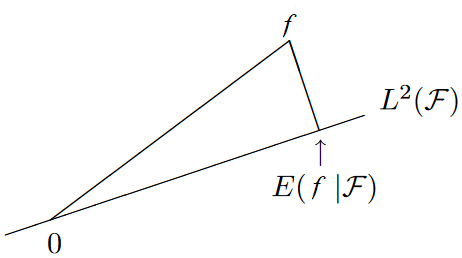
\includegraphics[scale=0.8]{img/projection.png}
		\caption{Conditional expectation as projection in $L^{2}$.}
	\end{figure}
	
	
	
	
	
	\section{Markov Chains}
	
	
	\begin{defn}
		Let $h: X \to Y$ be a function from a set $X$ to a measurable space $(Y,\mathcal{G})$. We define on $X$ the \textit{$\sigma$-algebra generated by $h$} to be the smallest $\sigma$-algebra with respect to which $h$ is measurable:
		\begin{equation*}
			\sigma(h) := \{h^{-1}(A);\, A \in \mathcal{G}\}.
		\end{equation*}
		If $\{(Y_{\alpha},\mathcal{G}_{\alpha}),\; \alpha \in \Gamma\}$ is a family of measurable spaces and $\mathcal{C} := \{h_{\alpha};\, \alpha \in \Gamma\}$ is a family of functions $h_{\alpha}: X \to Y_{\alpha}$, we then define the \textit{$\sigma$-algebra generated by $\mathcal{C}$} to be:
		\begin{equation*}
			\sigma(h_{\alpha};\, \alpha \in \Gamma) := \sigma\left(\bigcup_{\alpha\in\Gamma}\sigma(h_{\alpha})\right).
		\end{equation*}
	\end{defn}


    \begin{defn}\label{definition independence}
        Let $(X, \mathcal{F}, \mu)$ be a probability space.
        \begin{itemize}
            \item Two sets $A, B \in \mathcal{F}$ are \textit{independent} if $\mu(A\cap B) = \mu(A)\mu(B)$.
            \item Two $\sigma$-algebras $\mathcal{F}, \mathcal{G}$ are \textit{independent} if, for every $A \in \mathcal{F}$ and $B \in \mathcal{G}$, $A$ and $B$ are independent.
            \item A random variable $h: X \to \R$ is \textit{independent} of the $\sigma$-algebra $\mathcal{G}$ if $\sigma(f)$ is independent of $\mathcal{G}$.
            \item Two random variables $h_{1},h_{2}: X \to \R$ are \textit{independent} if their generated $\sigma$-algebras $\sigma(h_{1})$ and $\sigma(h_{2})$ are independent.
            \item A sequence $(h_{n})_{n\in\N_{0}}$ of random variables is \textit{independent} if any finite sub-collection of them is independent, in the following sense:
            \begin{equation*}
                \mu\left(\bigcap\limits_{j=1}^{k}h_{i_{j}}^{-1}(A_{i_{j}})\right) = \prod\limits_{j=1}^{k}\mu\left(h_{i_{j}}^{-1}(A_{i_{j}})\right),
            \end{equation*}
            for any finite subset $\{i_{1},\dots,i_{k}\} \subset \N_{0}$ and $A_{i_{j}} \in \mathcal{B}(\R)$.
        \end{itemize}
    \end{defn}

    \begin{prop}
        If $h_{1}$ and $h_{2}$ are independent random variables, then $\mathbb{E}(h_{1}h_{2}) = \mathbb{E}(h_{1})\mathbb{E}(h_{2})$. Also, if $h: X \to \R$ is independent of a $\sigma$-algebra $\mathcal{G}$, then $\mathbb{E}(h|\mathcal{G}) = \mathbb{E}(h)$ almost everywhere.
        \begin{proofqed}
            First consider the case of indicator functions, $h_{1} = \chi_{A}$ and $h_{2} = \chi_{B}$. Then:
            \begin{equation*}
                \mathbb{E}(\chi_{A}\chi_{B}) = \int\chi_{A}\chi_{B}\,d\mu = \int_{A\cap B}\,d\mu = \mu(A\cap B) = \mu(A)\mu(B) = \int\chi_{A}\,d\mu\int\chi_{B}\,d\mu = \mathbb{E}(\chi_{A})\mathbb{E}(\chi_{B}).
            \end{equation*}
            By linearity, the result follows for any elementary function and, by convergence theorems on Measure Theory, it follows also for any positive integrable function. Finally, summing up the positive and negative parts, the result is valid for any integrable function.

            For the second statement, let $A \in \mathcal{G}$ and define $h_{2} := \chi_{A}$. Then $h$ and $h_{2}$ are independent random variables. From the first part we have:
            \begin{equation*}
                \int_{A}\mathbb(E|\mathcal{G})\,d\mu = \int_{A}h\,d\mu = \mathbb{E}(h\chi_{A}) = \mathbb{E}(h)\mathbb{E}(\chi_{A}) = \mathbb{E}(h)\mu(A) = \int_{A}\mathbb{E}(h)\,d\mu. \eqno\qedsymbol
            \end{equation*}
        \end{proofqed}
    \end{prop}
    
 \newpage


	Let $M$ be a metric space with the Borel $\sigma$-algebra $\mathcal{B}(M)$, and $(\Omega, \mathcal{F}, \mathbb{P})$ a probability space.
	
	
	
	\begin{defn}
		A function $p: M \times \mathcal{B}(M) \to \R$ is said to be a \textit{transition probability} if:
		\begin{enumerate}
			\item For each $x \in M$, the function $A \mapsto p(x,A)$ is a probability measure on $(M, \mathcal{B}(M))$;
			\item For each $A \in \mathcal{B}(M)$, the function $x \mapsto p(x,A)$ is measurable.
		\end{enumerate}
	\end{defn}
	
	\begin{defn}
		Let $I$ be a subset of $\R$. A \textit{stochastic process} is a family $Z = \{Z_{t};\, t \in I\}$ of random variables on $\Omega$ with values in $M$.
	\end{defn}
	
	\begin{rem}
		In this work we will consider only the case where $I = \N_{0}$.
	\end{rem}


	\begin{defn}
		Let $(Z_{n})_{n\in\N_{0}}$ be a stochastic process on $\Omega$ with values in $M$. We say that $(Z_{n})_{n\in\N_{0}}$ is a \textit{Markov chain with transition probability $p$} if, for every $A \in \mathcal{B}(M)$:
		\begin{equation}\label{def markov chain}
			\mathbb{P}(Z_{n+1} \in A \,|\, \mathcal{F}_{n}) = p(Z_{n},A).
		\end{equation}
		Here, $\mathcal{F}_{n} := \sigma(Z_{0},\dots Z_{n})$, and the notation $\mathbb{P}(Z_{n+1} \in A\,|\,\mathcal{F}_{n})$ means the conditional expectation (with respect to the measure $\mathbb{P}$) $\mathbb{E}\left(\chi_{Z_{n+1}^{-1}(A)}\,|\,\mathcal{F}_{n}\right)$. So \eqref{def markov chain} means that, for $\mathbb{P}$-almost every $\omega \in \Omega$:
		\begin{equation*}
			\mathbb{P}\left(Z_{n+1} \in A\,|\,\mathcal{F}_{n}\right)(\omega) = \mathbb{E}\left(\chi_{Z_{n+1}^{-1}(A)}\,|\,\mathcal{F}_{n}\right)(\omega) = p(Z_{n}(\omega),A).
		\end{equation*}
	\end{defn}
	

	\begin{rem}
		In the case where $M$ is countable, the Markov property is equivalent to say that, for all $z_{0}, \dots, z_{n}, z \in M$, we have:
		\begin{equation*}
			\mathbb{P}(Z_{n+1} = z \,|\, Z_{0}=z_{0},\dots,Z_{n}=z_{n}) = \mathbb{P}(Z_{n+1}=z\,|\,Z_{n}=z_{n}).
		\end{equation*}
		%for all $k \leq n$, all $n_{1} < \cdots < n_{k} < n+1$ and all $z_{1}, \dots, z_{k}, z \in M$, we have:
		%\begin{equation*}
		%	\mathbb{P}(Z_{n+1} = z \,|\, Z_{n_{1}}=z_{1},\dots,Z_{n_{k}}=z_{k}) = \mathbb{P}(Z_{n+1}=z\,|\,Z_{n_{k}}=z_{k}).
		%\end{equation*}
	\end{rem}


\quad


    \begin{defn}
        Let $(X,\mathcal{F},\mu)$ be a probability space and $(Y,\mathcal{G})$ a measurable space. If $h: X \to Y$ is a measurable function, we can define the \textit{push-forward measure} $h_{*}\mu$ on $Y$ by:
        \begin{equation*}
            h_{*}\mu(A) := \mu(h^{-1}(A)) ~~~~ \forall\, A \in \mathcal{G}.
        \end{equation*}
        We call $h_{*}\mu$ the \textit{distribution} of $h$.
    \end{defn}

    \begin{rem}
        We say that a stochastic process $(X_{n})_{n\in\N_{0}}$ is \textit{independent and identically distributed (i.i.d.)} if it is independent, in the sense of Definition~\ref{definition independence}, and each $X_{n}$ has the same distribution $(X_{n})_{*}\mu = \nu$.
    \end{rem}

    \begin{example}
        Given a measurable space $(Y,\mathcal{G})$ and a point $y \in Y$, we can define the \textit{Dirac Delta measure} on $Y$:
        \begin{equation*}
            \delta_{y}(A) := \left\{\begin{array}{ll}
                 1 & \text{ if } y \in A, \\
                 0 & \text{ if } y \not\in A
            \end{array}\right. ~~~~ \forall\, A \in \mathcal{G}.
        \end{equation*}
    \end{example}
 
		
	
	\section{Stationary Measures}
	
	Let $(\Omega, \mathcal{F}, \mathbb{P})$ be a probability space, and $X = (X_{n})_{n\in\N_{0}}$ an independent stochastic process on $\Omega$ with values on a finite set $\{1,\dots,k\}$, such that each $X_{n}$ has the same distribution $\nu = p_{1}\delta_{1} + \cdots + p_{k}\delta_{k}$. Let $Z_{0}$ be a random variable on $\Omega$ with values in a metric space $M$ independent of $X$.
	
	Consider $f_{1},\dots, f_{k}: M \to M$ to be continuous functions, and define the sequence of random variables:
	\begin{equation*}
		Z_{n}(\omega) := f_{X_{n-1}(\omega)}\circ \cdots \circ f_{X_{0}(\omega)}(Z_{0}(\omega)) = f_{X_{n-1}}(Z_{n-1}).
	\end{equation*}

	\begin{prop}
		The sequence $(Z_{n})_{n\in\N_{0}}$ is a Markov chain with transition probability given by:
		\begin{equation*}
			p(x,A) = \int\chi_{A}(f_{i}(x))\,d\nu(i) = \sum_{i=1}^{k}p_{i}\,\chi_{A}(f_{i}(x)).
		\end{equation*}
		\begin{proof}
			We need to prove that, for each $A \in \mathcal{B}(M)$ and $\mathbb{P}$-almost every $\omega \in \Omega$:
			\begin{equation*}
				\mathbb{P}\left(Z_{n+1} \in A \,|\, \sigma(Z_{0},\dots,Z_{n})\right)(\omega) = p(Z_{n}(\omega),A).
			\end{equation*}
			Remember: to prove that some conditional expectation $\mathbb{E}(f|\mathcal{G})$ is essentially equal to a function $g$ is the same as proving that $g$ is $\mathcal{G}$-measurable and that, for each $B \in \mathcal{G}$, we have $\int_{B}g = \int_{B}f$.
			
			\noindent\textbf{Step 1.} Given $B \in \sigma(Z_{0},\dots,Z_{n})$, we must prove that:
			\begin{equation}\label{formula 1 prop 3.1}
				\int_{B}\chi_{A}(Z_{n+1}(\omega))\,d\mathbb{P}(\omega) = \int_{B}p(Z_{n}(\omega),A)\,d\mathbb{P}(\omega).
			\end{equation}
			Observe that $\sigma(Z_{0},\dots,Z_{n}) \subset \sigma(Z_{0},X_{0},\dots,X_{n-1})$. In fact, we have the following compositions:
            \begin{equation*}
                \begin{array}{ccccc}
                    \Omega & \stackrel{(X_{0},\dots,X_{n-1},Z_{0})}{\longrightarrow} & \left\{1,\dots,k\right\}^{n} \times M & \stackrel{f}{\longrightarrow} & M \\
                    \omega & \longmapsto & \left(X_{0}(\omega),\dots,X_{n-1}(\omega),Z_{0}(\omega)\right) & \longmapsto & Z_{n}(\omega).
                \end{array}
            \end{equation*}
            Now take a basis set $B \in \sigma(Z_{0},\dots,Z_{n})$, $B \in \sigma(Z_{0})\cup\cdots\cup\sigma(Z_{n})$. If $B \in \sigma(Z_{0})$, then of course it belongs to $\sigma(Z_{0},X_{0},\dots,X_{n-1})$. Suppose that $B \in \sigma(Z_{j})$, $j \neq 0$. Then $B = Z_{j}^{-1}(C)$ for some $C \in \mathcal{B}(M)$. By the above composition, we also have $B = Z_{j}^{-1}(C) = (X_{0},\dots,X_{n-1},Z_{0})^{-1}(f^{-1}(C)) \in \sigma(X_{0},\dots,X_{n-1},Z_{0})$; this concludes the claim.
   
            We also know, as above, that $\sigma(Z_{0},X_{0},\dots,X_{n-1})$ is the $\sigma$-algebra generated by the following map $\iota: \Omega \to \{1,\dots,k\}^{n}\times M$:
			\begin{equation*}
				\iota(\omega) := \left(X_{0}(\omega),\dots,X_{n-1}(\omega),Z_{0}(\omega)\right).
			\end{equation*}
			So $B$ can be chosen as a set of the form $\iota^{-1}(B')$ for some measurable set $B'$ on $\{1,\dots,k\}^{n}\times M$. We then have:
			\begin{eqnarray*}
				\int_{B}\chi_{A}(Z_{n+1})\,d\mathbb{P} &=& \int\chi_{A}(Z_{n+1})\,\chi_{B}\,d\mathbb{P} \\
				&=& \int\chi_{A}(f_{X_{n}}\circ\cdots\circ f_{X_{0}}(Z_{0}))\,\chi_{B'}(X_{0},\dots,X_{n-1},Z_{0})\,d\mathbb{P}.
			\end{eqnarray*}
			Since $X_{0},\dots,X_{n},Z_{0}$ are independent, the distribution of the vector $(X_{0},\dots,X_{n},Z_{0})$ is $\nu^{n+1}\times\mu$. Denoting by $(\alpha_{0},\dots,\alpha_{n},x)$ a typical vector on $\{1,\dots,k\}^{n+1}\times M$, we then have:
			\begin{equation}\label{formula 2 prop 3.1}
				\int_{B}\chi_{A}(Z_{n+1})\,d\mathbb{P} = \iint\chi_{A}(f_{\alpha_{n}}\circ\cdots\circ f_{\alpha_{0}}(x))\,\chi_{B'}(\alpha_{0},\dots,\alpha_{n-1},x)\,d\nu^{n+1}d\mu.
			\end{equation}
			Moreover, by definition of $p$, we know that:
			\begin{equation*}
				\int\chi_{A}(f_{\alpha_{n}}\circ\cdots\circ f_{\alpha_{0}}(x))\,d\nu(\alpha_{n}) = p(f_{\alpha_{n-1}}\circ\cdots\circ f_{\alpha_{0}}(x),A).
			\end{equation*}
			From \eqref{formula 2 prop 3.1} we obtain:
			\begin{eqnarray*}
				\int_{B}\chi_{A}(Z_{n+1})\,d\mathbb{P} &=& \int p(f_{\alpha_{n-1}}\circ\cdots\circ f_{\alpha_{0}}(x),A)\chi_{B'}(\alpha_{0},\dots,\alpha_{n-1},x)\,d\nu^{n}d\mu \\
				&=& \int_{B}p(f_{X_{n-1}}\circ\cdots\circ f_{X_{0}}(Z_{0}),A)\,d\mathbb{P}.
			\end{eqnarray*}
			This proves formula \eqref{formula 1 prop 3.1}, concluding the first step.
			
			\noindent\textbf{Step 2.} We now prove that the function $p(Z_{n},A): \Omega \to \R$ is $\sigma(Z_{0},\dots,Z_{n})$-measurable. Since $A \in \mathcal{B}(M)$ is fixed, we have the following compositions.
			\begin{equation*}
				\begin{array}{ccccc}
					\Omega &\longrightarrow& M & \longrightarrow& \R \\
					\omega &\longmapsto &Z_{n}(\omega)& \longmapsto &p(Z_{n}(\omega),A).
				\end{array}
			\end{equation*}
			By definition of transition probability, the second arrow is a measurable function. The first arrow is $\sigma(Z_{n})$-measurable by definition of generated $\sigma$-algebra; since $\sigma(Z_{n}) \subset \sigma(Z_{0},\dots,Z_{n})$, we know that it is also $\sigma(Z_{0},\dots,Z_{n})$-measurable. Finally, the composition of measurable functions is also measurable, and we conclude the proof.
		\end{proof}
            \end{prop}

%-------------------------------------------------%

\subsection{Stationary Measure}

In this part our goal is to that prove the previously Markov Chain has a stationary measure. 
For that, let $(M,d)$ be a metric space and $\mathcal{M}_1(M)$ be the set of all probability measures on $M$. 

Suppose $Z_0$ has distribution $\mu$, then the distribution of $Z_n$ is $\mathcal{T}^n  \mu$, with 
\begin{align*}
    \mathcal{T}:\mathcal{M}_1(M) &\to \mathcal{M}_1(M)\\
    \mu &\mapsto \mathcal{T}\mu (A) = \int p(x,A) d\mu(x)
\end{align*}
being the Markov Operator.

In fact, suppose $Z_n$ has distribution $\nu$ so the distribution of $Z_{n+1}:\Omega\to M$ can be define by $Z_{n+1}*\mathbb{P}$ such that 
$$Z_{n+1}*\mathbb{P}(A) = \mathbb{P}(Z_{n+1}^{-1}(A)) = \mathbb\{w \in \Omega: Z_1(\omega) \in A\} = \mathbb{P}(Z_{n+1} \in A).$$

We already saw that 
\begin{align*}
    Z_{n+1}*\mathbb{P}(A) = \mathbb{P}(Z_{n+1} \in A) 
    = \int \chi_A(Z_{n+1}(\omega))d\mathbb{P}(\omega)
    = \int p(Z_n(\omega,A) d\mathbb{P}(\omega)
    = \int p(x,A) dZ_n*\mathbb{P}(x)
    = \int p(x,A) d\nu(x).
\end{align*}
A measure $\mu$ is said to be stationary measure if $Z_0$ has distribution $\mu$ then so does $Z_n$ for all $n \geq 1$. In other words, $\mu$ is a fixed point for the Markov Operator.

So to be able to determine the stationary measure we need first define a topology for $\mathcal{M}_1(M)$ called by Weak* Topology. 

\subsection{Weak* topology}
    To define the Weak* topology in the probability measures set, we need to see the following definitions.

    \begin{defn}
        Given $B \subset M$, we call the $\delta-$neighborhood of $B$ the set 
        $$ B^{\delta} = \{x \in M: d_1(x,B) < \delta\},$$
    with $d_1(x,B) = \inf\{d(x,b): b \in B\}$.
    \end{defn}

    \begin{defn}
        Given $\mu \in \mathcal{M}_1(M)$, $\epsilon>0$ and $\Phi = \{\phi_i: i=1,\dots,N\}$ such that 
        $$ \phi_i: M \to \mathbb{R}, \forall i=1,\dots,N$$
    are bounded continuous functions. Define the set 
    $$ V(\mu,\Phi,\epsilon) =\{ \nu \in \mathcal{M}_1(M): \left|\int \phi_i d\nu - \int \phi_i d\mu \right| < \epsilon, \,\,\, \forall i=1,\dots,N\}.$$
    \end{defn}

    \begin{prop}
        The family $\mathcal{B} = \{V(\mu,\Phi,\epsilon)\}$  may be taken as a base for a topology in $\mathcal{M}_1(M)$.
        

        \proof To prove that it's sufficient to show the following two conditions:
        \begin{itemize}
            \item each $\nu \in \mathcal{M}_1(M)$ is contained in some subset in $\mathcal{B}$;
            \item if $V_1,V_2 \in \mathcal{B}$ and $\nu \in V_1 \cap V_2$, then exists $W \in \mathcal{B}$ with $\nu \in \mathcal{B} \subset V_1 \cap V_2$. 
        \end{itemize}

        In fact, by definition  $\nu \in V(\nu, \Phi, \epsilon)$ for every $\Phi$ and $\epsilon>0$. 

        Moreover, consider $\nu \in V(\mu_1, \Phi_1, \epsilon_1) \cap V(\mu_2, \Phi_2, \epsilon_2)$ with $\Phi_1 = \{\phi_{1i}: i=1,\dots,N_1\}$,
        $\Phi_2 = \{\phi_{2i}: i=1,\dots,N_2\}$ and $\epsilon_1,\epsilon_2>0$.
        
        Then
        $$ \left| \int \phi_{1i} d\nu - \int \phi_{1i} d\mu_1\right| < \epsilon, \,\,\, \forall i=1,\dots,N_1$$
and 
        $$ \left| \int \phi_{2i} d\nu - \int \phi_{2i} d\mu_2\right| < \epsilon, \,\,\, \forall i=1,\dots,N_2.$$

        Consider 
        $$ r_1 = \max\left\{ \left| \int \phi_{1i} d\nu - \int \phi_{1i} d\mu_1\right|: i=1,\dots,N_1\right\}$$
    and
        $$ r_2 = \max\left\{ \left| \int \phi_{2i} d\nu - \int \phi_{2i} d\mu_2\right|: i=1,\dots,N_2\right\}$$

        Taking $\epsilon = \min\{\dfrac{\epsilon_1-r_1}{2}, \dfrac{\epsilon_2-r_2}{2}\}$  and $\Phi = \Phi_1 \cup \Phi_2$, 
        define the set $V(\nu, \Phi, \epsilon)$. 

        If $z \in V(\nu, \Phi, \epsilon)$ then 
        $$ \left| \int \phi_{1i} dz - \int \phi_{1i} d\nu \right| < \epsilon, \,\,\, \forall i=1,\dots,N_1$$
 therefore 
        \begin{align*}
        \left| \int \phi_{1i} dz - \int \phi_{1i} d\mu_1 \right| &\leq 
        \left| \int \phi_{1i} dz - \int \phi_{1i} d\nu \right|
        +
        \left| \int \phi_{1i} d\nu - \int \phi_{1i} d\mu_1 \right|\\
        &< \epsilon + r_1\\
        &<\epsilon_1
        \end{align*}
that means $z \in V(\mu_1, \Phi_1, \epsilon_1)$.

    With a similar process we get $z \in V(\mu_2, \Phi_2, \epsilon_2)$.
        
    \end{prop}
    
\begin{defn}[Weak* topology] The weak* topology it's the topology generated by $\mathcal{B}$.
\end{defn}

\begin{lemma}[Convergence in $\mathcal{M}_1(M)$]
    A sequence $(\mu_n)_{n \in \mathbb{N}}$ of $\mathcal{M}_1(M)$ elements converges to a measure $\mu \in \mathcal{M}_1(M)$ in the weak* topology if and only if 
    $$ \int \phi d\mu_n \to \int \phi d\mu \,\,\forall \text{ bounded continuous functions } \phi:M \to \mathbb{R}.$$

    \proof ($\Longrightarrow$) Suppose $\mu_n \to \mu$ in the weak* topology, consider any $\phi:M \to \mathbb{R}$ bounded continuous function and the set $\Phi = \{\phi\}$.

    So for any $\epsilon>0$ there is a $n_0 \in \mathrm{N}$ that 
    $$\mu_n \in V(\mu, \Phi, \epsilon), \forall n \geq n_0.$$

    In other way: 
    $$ \left| \int \phi d \mu_n - \int \phi d \mu \right| < \epsilon, \,\, \forall n_0 \leq n,$$
and that implies 
    $$\int \phi d \mu_n \to \int \phi d \mu$$
in $\mathbb{R}$.

($\Longleftarrow$) Suppose that  $\int \phi d \mu_n \to \int \phi d \mu$ in $\mathbb{R}$ for all bounded continuous function $\phi:M \to \mathbb{R}$. 

    Given any $\Phi = \{\phi_i: i=1,\dots,N\}$ and $\epsilon>0$, so for every $i=1,\dots,N$ exists $n_0^i \in \mathrm{N}$ such that 
    $$ n > n_0^i \implies \left|  \int \phi_i d \mu_n - \int \phi_i d \mu \right| < \epsilon.$$

    Choosing $n_0 = \max\{n_0^i: i=1,\dots,N\}$ we have 
    $$ n > n_0 \implies \left|  \int \phi_i d \mu_n - \int \phi_i d \mu \right| < \epsilon, \,\,\, \forall i=1,\dots,N$$
and that implies 
    $$\mu_n \in V(\mu,\Phi, \epsilon),\,\,\, \forall n>n_0.$$

    Therefore $\mu_n \overset{*}{\to} \mu$ in weak* topology.
\end{lemma}

\subsection{Markov Operator}

The Markov Operator is define by:
\begin{align*}
    \mathcal{T}:\mathcal{M}_1(M) &\to \mathcal{M}_1(M)\\
    \mu &\mapsto \mathcal{T}\mu (A) = \int p(x,A) d\mu(x). 
\end{align*}

    Consider the Markov Chain $(Z_n)$ previously defined, if $Z_0$ has distribution $\mu$ then the distribution of $Z_n$ is given by $\mathcal{T}^n \mu$.

    \begin{defn} The distribution $\mu$ on $M$ is called stationary measure if it is a fixed point of the Markov Operator.
    \end{defn}
    
    \begin{prop}
    If $\phi:M \to \mathbb{R}$ is a bounded continuous function, then 
    $$ \int \phi(y) p(x,dy) = \sum_{i=1}^{k}p_i \phi \circ f_i(x).$$

    And denote $P \phi(x) = \int \phi(y) p(x,dy)$.
    
    \proof Remember that 
    $$p(x,A) = \int \chi_A(f_i(x))d\nu(i) = \sum_{i=1}^{k}p_i \chi_A(f_i(x)).$$ 
    
    We will divide this proof in four steps. 

    \textbf{Step 1.} Suppose that $\phi$ is a characteristic function, that is, $\phi = \chi_B$, for some $B \subset M$. So
    \begin{align*}
        \int \phi(y) p(x,dy) &= \int \chi_B(y) p(x,dy) \\
        &=  p(x,B) \\
        &= \int \chi_B(f_i(x))d\nu(i)\\
        &= \sum_{i=1}^{k}p_i \chi_B(f_i(x))\\
        &= \sum_{i=1}^{k}p_i \phi(f_i(x))
    \end{align*}

    \textbf{Step 2.} Suppose that $\phi$ is a simple function, that is, 
    $\phi = \sum_{j=1}^{m} \alpha_j \chi_{A_j}$, with $M=\displaystyle\cup_{j=1}^{m} A_j$ and $A_j\cap A_K =\varnothing$. So 
    \begin{align*}
        \int \phi(y) p(x,dy) &= \int \sum_{j=1}^{m} \alpha_j \chi_{A_j} p(x,dy) \\
        &=  \sum_{j=1}^{m} \alpha_j  \int  \chi_{A_j} p(x,dy) \\
        &=  \sum_{j=1}^{m} \alpha_j  \sum_{i=1}^{k}p_i \chi_{A_j}(f_i(x)) \\
        &=  \sum_{i=1}^{k}p_i \sum_{j=1}^{m} \alpha_j \chi_{A_j}(f_i(x)) \\
        &= \sum_{i=1}^{k} p_i \phi(f_i(x)).
    \end{align*}

    \textbf{Step 3.} Suppose that $\phi$ is a positive function. So there is a sequence of samples functions $(s_n)_n$ that $s_1 \leq s_2 \leq \dots \leq \phi$. 

    We know that 
    $$\int \phi(y) p(x,dy) = \sup \Big\{ \int s_n(y) p(x,dy): n \in \mathbb{N}\Big\}.$$

    For the step 2 we have:
    \begin{align*}
    \int \phi(y) p(x,dy) &= \sup \Big\{ \sum_{i=1}^{k} p_i s_n \circ f_i(x) : n \in \mathbb{N}\Big\} \,\,\,\,(\sup s_n = \phi)\\
    &= \sum_{i=1}^{k} p_i \phi \circ f_i(x)
    \end{align*}

    \textbf{Step 4.} Let $\phi$ be any function, so $\phi = \phi^+ - \phi^-$ where $\phi^+$ and $\phi^-$ are positive functions, so 
    \begin{align*}
     \int \phi(y) p(x,dy) &=\int \phi^+(y) p(x,dy) - \int \phi^-(y) p(x,dy) \,\,\,\,\,(\text{Step 3})\\
     &=\sum_{i=1}^{k} p_i \phi^+(f_i(x)) - \sum_{i=1}^{k} p_i \phi^-(f_i(x))\\
     &=\sum_{i=1}^{k}p_i ( \phi^+(f_i(x)) - \phi^-(f_i(x))) \\
     &= \sum_{i=1}^{k} p_i \phi \circ f_i(x).
    \end{align*}
    \end{prop}

    \textbf{Affirmation.} If $\Phi:M \to \mathbb{R}$ it's a integral function so 
    $\int \phi d\mathcal{T}\mu = \int \phi(y) \int p(x,dy) d\mu_n(x) = \int \int \phi(y) p(x,dy) d \mu(x).$

    In fact, we will to show this affirmation in four steps.

    \textbf{Step 1.} Suppose $\phi = \chi_B$ for some $B \subset M$ measurable, then 
    \begin{align*}
    \int \phi d\mathcal{T}\mu 
    &= \int \chi_B(y) d\mathcal{T}\mu = \mathcal{T}\mu(B) \\
    &= \int p(x,B) d\mu(x)\\
    &= \int \int \chi_B(y) p(x,dy) d\mu(x)\\
    &= \int \int \phi(y) p(x,dy) d\mu(x).
    \end{align*}

    \textbf{Step 2.} Suppose $\phi$ is a simple function, that is, 
    $\phi = \sum_{j=1}^{m} \alpha_j \chi_{A_j}$, with $M=\displaystyle\cup_{j=1}^{m} A_j$ and $A_j\cap A_K =\varnothing$, then
    \begin{align*}
    \int \phi d\mathcal{T}\mu 
    &= \int \sum_{j=1}^{m} \alpha_j \chi_{A_j} d\mathcal{T}\mu 
    = \sum_{j=1}^{m} \alpha_j \mathcal{T}\mu(A_j)  \\
    &=\sum_{j=1}^{m} \alpha_j \int p(x,A_j) d\mu(x)\\
    &= \int \sum_{j=1}^{m} \alpha_j p(x,A_j) d\mu(x)\\
    &= \int \int \phi(y) p(x,dy) d\mu(x).
    \end{align*}

    \textbf{Step 3.} Suppose that $\phi$ is a positive function. So there is a sequence of samples functions $(s_n)_n$ that $s_1 \leq s_2 \leq \dots \leq \phi$. 
    \begin{align*}
    \int \phi d\mathcal{T}\mu &=  \sup \Big\{ \int s_n(y) d\mathcal{T}\mu: n \in \mathbb{N}\Big\}\\
    &=\sup \Big\{ \int \int s_n(y) p(x,dy) d\mu(x): n \in \mathbb{N}\Big\}\\
    &=\int \int \phi(y) p(x,dy) d\mu(x).
    \end{align*}

    \textbf{Step 4.} If $\phi$ be any function, so $\phi = \phi^+ - \phi^-$ where $\phi^+$ and $\phi^-$ are positive functions and the prove is immediately from the previously step.
    
    \begin{prop}\label{Convergence fixed point}
        If $\mu_n \overset{*}{\to} \mu$ (that is $\mu_n$ converges to $\mu$ in the weak* topology), then  
        $\mathcal{T}\mu_n \overset{*}{\to} \mathcal{T}\mu$.

        \proof For the hypothesis $\mu_n \overset{*}{\to} \mu$ implies that for any continuous bounded function $\phi:M \to \mathbb{R}$ we have
        $$ \lim_{n \to \infty} \int \phi d\mu_n = \int \phi d\mu.$$

        By the other side 
        $$\int \phi d\mathcal{T}\mu_n = \int \phi(y) \int p(x,dy) d\mu_n(x) = \int \int \phi(y) p(x,dy) d \mu_n(x).$$

        \textbf{Afirmation. }
        We already showed that 
        $$ P\phi(x) = \int \phi(y) p(x,dy) = \sum_{i=1}^{k} p_i \phi \circ f_i(x)$$
    because $f_i$ ($\forall i=1,\dots,k$), $\phi$ are continuous and $\phi$ is bounded we have $P\phi(y)$ also is a bounded and continuous function. 

        Therefore, 
        \begin{align*}
         \lim \int \phi(y) d\mathcal{T}\mu_n(y) 
         &= \lim \int \phi(y) \int  p(x,dy) d \mu_n(x) \\
         &= \lim \int \int \phi(y) p(x,dy) d \mu_n(x) \\
         &= \lim \int P\phi(x) d \mu_n(x) \\
         &= \int P\phi(x) d \mu(x) \\
         &= \int \int \phi(y) p(x,dy) d \mu(x)\\
         &= \int \phi(y) \int \ p(x,dy) d \mu(x)\\
         &=\int \phi(y) d\mathcal{T}\mu(y).
        \end{align*}

        That means $\mathcal{T}\mu_n \overset{*}{\to} \mathcal{T}\mu$.
    \end{prop}

    \begin{defn}
        Let $\pi:\Omega \to M$ be defined by 
        $$ \pi(\omega) = \lim_{n \to \infty} f_{\omega_0} \circ \cdots \circ f_{\omega_n}(p).$$

        The pushforward measure $\pi_*\mathbb{P} $  in $M$ is defined by 
        $$\pi_*\mathbb{P}(A) = \mathbb{P}(\pi \in A) = \mathbb(\{\omega: \pi(\omega) \in A\}). $$

    \end{defn}

    \subsubsection{Letac Principle}
    \begin{prop}[Letac Principle] 
    Consider an independent and identically distributed random product of continuous functions $f_{1},\cdots, f_{k}:M\rightarrow M$. Suppose the limit 
    $$\pi(\omega) = \lim_{n \to \infty} f_{\omega_0} \circ \cdots \circ f_{\omega_n}(p)$$
    exists for $\mathbb{P}-$almost every point $\omega \in \Omega$ and it is independent of $p \in M$.

    Then for every $\nu \in \mathcal{M}_1(M)$ we have 
    $$ \mathcal{T}^n \nu \overset{*}{\to} \pi_*\mathbb{P}.$$

    In particular, $\pi_*\mathbb{P}$ it's a stationary measure.
    
    \proof We want to show that for every bounded continuous function $\phi:M \to \mathbb{R}$ is true
    $$ \lim_{n \to \infty}\int \phi d\mathcal{T}^n\nu = \int \phi d\pi_*\mathbb{P}.$$

    Because $\pi_*\mathbb{P}$ is a pushforward measure we know that for every $B \in \mathcal{B}(M)$ 
    \begin{align*}
        \int_B \phi d\pi_*\mathbb{P} 
        &= \int_{\pi^{-1}(B)} \phi(\pi(\omega)) d\mathbb{P}(\omega)\\
        &= \int_{\pi^{-1}(B)} \phi(\lim_{n \to \infty} f_{\omega_0} \circ \cdots \circ f_{\omega_n}(p)) d\mathbb{P}(\omega)\\
    \end{align*}
by the hypothesis $\phi$ is continuous 
    \begin{align*}
        \int_B \phi d\pi_*\mathbb{P} 
        &= \lim_{n \to \infty} \int_{\pi^{-1}(B)} \phi( f_{\omega_0} \circ \cdots \circ f_{\omega_n}(p)) d\mathbb{P}(\omega)\\
    \end{align*}
and 
    \begin{align*}
        \int \phi d\pi_*\mathbb{P} 
        &= \lim_{n \to \infty} \int \phi( f_{\omega_0} \circ \cdots \circ f_{\omega_n}(p)) d\mathbb{P}(\omega).
    \end{align*}

    By the other side 
    $$ \int \phi(f_{\omega_0}(x)) d\mathbb{P}(\omega) = \sum_{i=1}^{k} p_i \phi(f_i(x)).$$

    Furthermore  $P \phi(x) = \int \phi(y) p(x,dy) =\displaystyle\sum_{i=1}^{k}p_i \phi \circ f_i(x)$, that means 
    $$P \phi(x) = \int \phi(f_{\omega_0}(x)) d\mathbb{P}(\omega).$$

    In addiction, 
    \begin{align*}
       P^2 \phi(x) &= P (P \phi(x))\\
       &= \sum_{i=1}^{k} p_i P (\phi \circ f_i (x) )\\
       &= \sum_{i=1}^{k} p_i \displaystyle\sum_{j=1}^{k}p_j \phi \circ f_i \circ f_j(x)\\
       &= \sum_{i=1}^{k}\sum_{j=1}^{k} p_i p_j \phi ( f_i \circ f_j(x))\\
       &=\int \phi(f_{\omega_0}\circ f_{\omega_1}(x)) d\mathbb{P}(\omega)
    \end{align*}

    And by induction 
    $$ P^n \phi(x) =\int \phi(f_{\omega_0}\circ \dots \circ f_{\omega_n}(x)) d\mathbb{P}(\omega)$$
and 
    \begin{align*}
    \lim_{n \to \infty} P^n \phi(x) 
    &=\lim_{n \to \infty} \int \phi(f_{\omega_0}\circ \dots \circ f_{\omega_n}(x)) d\mathbb{P}(\omega)\\
    &= \int \phi(\lim_{n \to \infty} f_{\omega_0}\circ \dots \circ f_{\omega_n}(x)) d\mathbb{P}(\omega)\\
    &=\int \phi d\pi_*\mathbb{P}.
    \end{align*}

    Soon 
    \begin{align*}
    \int \phi(x) d\mathcal{T}^n\nu(x) = \int P^n \phi(x) d\nu(x) 
    \end{align*}
that implies 
    \begin{align*}
    \lim_{n \to \infty} \int \phi(x) d\mathcal{T}^n\nu(x) 
    &= \lim_{n \to \infty} \int P^n \phi(x) d\nu(x) \\  
    &= \int \lim_{n \to \infty} P^n \phi(x) d\nu(x) \,\,\,\,\,\,(P^n \phi \text{ continuous and bounded})\\  
    &= \int \int \phi d\pi_*\mathbb{P} d\nu(x) \,\,\,\,\,\,(\int \phi d\pi_*\mathbb{P} \text{ don't depend on }x)\\
    &= \int \phi d\pi_*\mathbb{P} \nu(M)\\
    &= \int \phi d\pi_*\mathbb{P}.
    \end{align*}

    Finally, $\pi_*\mathbb{P}$ it's a fixed point for $\mathcal{T}$. In fact, by the proposition \ref{Convergence fixed point} we have that 
    $$\mathcal{T}^n (\pi_*\mathbb{P}) \overset{*}{\to} \pi_*\mathbb{P}$$ 
    implies 
    $$\mathcal{T}^{n+1} (\pi_*\mathbb{P}) \overset{*}{\to} \mathcal{T}(\pi_*\mathbb{P}).$$

    And by the uniqueness of the limit $\mathcal{T}(\pi_*\mathbb{P}) = \pi_*\mathbb{P}$.

    Now suppose there are other fixed point $\nu$, that is $\mathcal{T}(\nu) = \nu$ which implies $\mathcal{T}^n(\nu) = \nu$. For the other side 
    $$\nu =  \lim_{n \to \infty} \mathcal{T}^n(\nu) = \pi_*\mathbb{P}.$$
    \end{prop}

        \subsubsection*{Corollary Letac Principle}
  
       Let 
    \begin{itemize}
        \item $(M,d)$ be a metric space;
        \item $\mathcal{B}(M)$ be the Borel $\sigma$-algebra of $M$;
        \item $(\Omega, \mathcal{F}, \mathbb{P})$ a probability space
        \item $Z = \{Z_{n}: \Omega\to M;\, n \in \mathbb{N}_0\}$ be a stochastic process;
        \item $M^{\mathbb{N}}$ be the space of sequence of $M$ with the $\sigma$-algebra $\mathcal{B}^{\mathbb{N}}$
    \end{itemize}

    \begin{defn}[Stationary process] A stochastic process $Z = \{Z_{n};\, n \in \mathbb{N}_0\}$ is stationary if 
    $$ \mathbb P (\{\omega : (Z_0,Z_1, \dots,Z_n ) \in C\}) = \mathbb P (\{\omega : (Z_k,Z_{1+k}, \dots,Z_{n+k} ) \in C\})$$
for any $k\geq 1$, $n \geq 0$ and any $C \in  \mathcal{B}^{\mathbb{N}}$.
    \end{defn}

    
    \begin{defn}[Invariant event] Let $Z = \{Z_{n};\, n \in \mathbb{N}_0\}$ be a stationary process.
    \begin{itemize}
        \item $A \in \mathcal{F}$ it's \textbf{invariant} if exists $C \in \mathcal{B}^{\mathbb{N}}$ such that 
        $$ A = \{\omega : ( Z_k(\omega),Z_{k+1}(\omega), \dots  ) \in C\}\,\,\,\, \forall k \geq 0.$$

        \item $A \in \mathcal{F}$ it's \textbf{almost invariant} if exists $B$ invariant such that 
        $$\mathbb P(A \triangle B) = 0.$$
    \end{itemize}
    \end{defn}

    \begin{defn}[Ergodicity] A stationary sequence $Z = \{Z_{n};\, n \in \mathbb{N}_0\}$ is ergodic if every invariant event has probability one or zero.       
    \end{defn}

    \begin{theorem}\label{Markov Ergodic} Suppose $\{X_n: n \geq 0\}$ is a stationary Markov process on a state space $(M, \mathbf{B}(M))$, with a transition probability $p(x,B)$ and a invariant initial distribution $m$. 

    The process is ergodic if and only if there does not exist an invariant distribution $\nu \neq m$ such that $\nu << m$.

    \proof \textcolor{red}{Working}
        
    \end{theorem}
    \begin{lemma} Let $Z = \{Z_{n};\, n \in \mathbb{N}_0\}$ be a Markov Chain with transition probability $p: M \times \mathcal{B}(M) \to \mathbb R$, and a unique stationary measure $m$. If $Z_0$ has distribution $m$, then $Z$ it's a stationary and ergodic process.

    \proof
    (Stationary Process) 
    
    \textbf{Affirmation.} 
    $$ \mathbb{P}(Z_i \in B_i, 0 \leq i \leq n ) = \int_{B_0} d Z_0 * \mathbb P \int_{B_1} p(x_0,dx_1) \cdots \int_{B_n} p(x_{n-1},dx_n).$$

    In fact, 
    \begin{itemize}
        \item Let's see for $\mathbb{P}(Z_0 \in B_0, Z_1 \in B_1) $.
        \begin{align*}
        \mathbb{P}(Z_0 \in B_0, Z_1 \in B_1) 
       & = \int \chi_{Z_1^{-1}(B_1)} \chi_{Z_0^{-1}(B_0)} d\mathbb P\\    
       & = \int_{Z_0^{-1}(B_0)} \chi_{Z_1^{-1}(B_1)}  d\mathbb P  \\
       & = \int_{Z_0^{-1}(B_0)} \chi_{Z_1^{-1}(B_1)}  d\mathbb P \\
       & = \int_{Z_0^{-1}(B_0)} p(Z_0,B_1)  d\mathbb P \,\,\,(\text{page 15})\\
       & = \int_{B_0} p(x_0,B_1)  d\mathbb P * Z_0 \,\,\,(\text{change of variables})\\
       & = \int_{B_0} \int_{B_1} p(x_0,dx_1)  d\mathbb P * Z_0.
        \end{align*}
    \end{itemize}

    Using the affirmation we can show that $(Z_n)_n$ it's stationary. 
    \begin{align*}
\mathbb{P}(Z_i \in B_i, 0 \leq i \leq n ) 
&= \int_{B_0} d Z_0 * \mathbb P \int_{B_1} p(x_0,dx_1) \cdots \int_{B_n} p(x_{n-1},dx_n) \\
&= \int_{B_0}  \int_{B_1} \cdots \int_{B_n} p(x_{n-1},dx_n) \cdots
p(x_0,dx_1) d Z_0 * \mathbb P \\
&= \int_{B_0}  \int_{B_1} \cdots \int_{B_n} p(x_{n-1},dx_n) \cdots
p(x_0,dx_1) d m \\
&= \int_{B_0}  \int_{B_1} \cdots \int_{B_n} p(x_{n-1},dx_n) \cdots
p(x_0,dx_1) d Z_k * \mathbb P \\
&= \mathbb{P}(Z_{i+k} \in B_i, 0 \leq i \leq n ) 
    \end{align*}

    (Ergodic Process) Immediate of the theorem \ref{Markov Ergodic}.
    \end{lemma}
    
    \begin{theorem}[Birkhoff's Ergodic Theorem] Let $\{X_n: n \geq 0\}$ be a stationary sequence on the state space $M$ and $f:M \to \mathbb R$ a function such that $\mathbb E [f(X_0)] < \infty$, then 
    $$\lim_{n \to \infty} \dfrac{1}{n} \sum_{m=0}^{n-1} f(X_m)$$
    exists almost sure. 

    If $\{X_n\}$ is ergodic then 
    $$\lim_{n \to \infty} \dfrac{1}{n} \sum_{m=0}^{n-1} f(X_m) = \mathbb E [f(X_0)] $$
        
    \end{theorem}
    \begin{corollary}[Law of the Large Numbers] Consider a space complete space metric $M$ and an i.i.d random product of contractions 
    $$f_i:M\to M\,\,\,\forall i=1,\dots,k$$

    Then the stationary measure $m$ satisfies: 
    \begin{enumerate}
        \item the support of $m$ it's the Hutchinson attractor $\text{supp}(m) = K$. 
        \item For every $x \in M$ and $\mathbb{P}-$almost every $\omega \in \Omega$, 
        $$ \lim_{n \to \infty} \dfrac{1}{n} \sum_{i=0}^{n-1} \phi( f_{\omega_{i-1}} \circ \dots \circ f_{\omega_0}(x)) = \int \phi(x)dm(x),$$
        for every bounded continuous function $\phi:M \to \mathbb{R}.$
    \end{enumerate}

    \proof Consider the Markov Chain $Z_n:\Omega \to M$
    $$Z_n(\omega) = f_{\omega_{n-1}}\circ \dots \circ f_{\omega_{0}}(\omega).$$

    Follows from Letac Principle that exists only one stationary measure $m = \pi * \mathbb{P}$, where 
    $$ \pi(\omega) = f_{\omega_{0}}\circ \dots \circ f_{\omega_{n-1}}(p).$$

    For this Markov Chain we have 
    \begin{itemize}
        \item $\text{supp}(\pi * \mathbb{P}) = K.$

        In fact, remember that
        $$K = \lim_{l \to \infty} \overline{\{f^{n}_\omega(x): n \geq l\}},$$
with $f^{n}_\omega(x) = f_{\omega_{n-1}}\circ \dots \circ f_{\omega_{0}}$.

    For  every $\omega$ we have $\pi(\omega) \in K$, and by definition $y \in \text{supp}(m)$ if $\mu(V) > 0$ for any neighborhood $V$ of $y$, and this happen only if $y \in K$.

    Suppose the opposite, that is exists $V$, $y \in V$ such that $V \cap K = \varnothing$ and $m(V)>0$. 

    We also have 
    $$ m (K) = \mathbb{P}(\{\omega \in \Omega: \pi(\omega) \in K\}) = 1,$$
so that implies 
    $$m(K\cap V) = m(K) + m(V) > 1,$$
but $m(A)<1$ for all $A \in \mathcal{B}(M).$

    On the other way, take $y \in K$, and a neighborhood $V$ of $y$, then by the $\pi$ continuity $\pi^{-1}(V)$ is a open subset of $\Omega$, that means exists a cylinder $C_{i,a_0, \cdots, a_k} \subset \pi^{-1}(V)$. 

    Because $\mathbb P (C_{i,a_0, \cdots, a_k}) > 0$, then  $\mathbb P (\pi^{-1}(V)) = m(V) >0$.
    
    Hence $\text{supp}(\pi * \mathbb{P}) = K.$

    \item Suppose the Markov Chain $\{Z_n: n \geq 0\}$ the element $Z_0$ has distribution $m = \pi * \mathbb{P}$ (the stationary measure by the Letac Principle), then this Markov Chain it's a ergodic and stationary process. 

    Let $g:M \to \mathbb{R}$ be a integrable function, so follows from Birkhoff's Ergodic Theorem 
    $$\lim_{n \to \infty} \dfrac{1}{n} \sum_{i=0}^{n-1} g(f_{\omega_{n-1}}\circ \dots \circ f_{\omega_{0}}(Z_0(\omega))) = \int g dm,$$
    for $\mathbb{P}-$almost every $\omega\in \Omega$.
    
    \textbf{Proof 1.} If $\phi:M \to \mathbb{R}$ is a bounded continuous functions then $\phi$ it's integrable, so for every $x \in M$ suppose the Markov Chain $Z_n(\omega) = f_{\omega_{n-1}}\circ \dots \circ f_{\omega_{0}}(\omega)$ start with $Z_0(\omega) = x$.   

    The $Z_0$ it's independent of $Z_n$, for all $n \geq 1$. In fact, \textcolor{red}{to ask}
    
    \textbf{Proof 2.} Consider the bounded continuous functions $\phi:M \to \mathbb{R}$, $|\phi(x)| \leq L$ for all $x \in M$. 

    We want to prove that:
    \begin{align*}
        \forall \varepsilon > 0 \exists n_0 \in \mathbb{N}: 
        n > n_0 \implies 
        \left| 
\dfrac{1}{n} \sum_{i=0}^{n-1} \phi (f_{\omega_{i-1}}\circ \dots \circ f_{\omega_{0}}(x) ) - \int \phi dm
        \right| < \varepsilon.
    \end{align*}

    
        For that let see
    \begin{align*}
        \left| 
\dfrac{1}{n} \sum_{i=0}^{n-1} \phi (f_{\omega_{i-1}}\circ \dots \circ f_{\omega_{0}}(x) ) - \int \phi dm
        \right|
        \leq 
        \left| 
\dfrac{1}{n} \sum_{i=0}^{n-1} \phi (f^{i}_{\omega}(x) ) 
- 
\dfrac{1}{n} \sum_{i=0}^{n-1} \phi (Z_i(\omega) ) 
        \right|        
    +
    \left| 
\dfrac{1}{n} \sum_{i=0}^{n-1} \phi (Z_i(\omega) ) 
- 
\int \phi dm
        \right|           
    \end{align*}

    We already know the last part converges, that is 
        \begin{align*}
    \left| 
\dfrac{1}{n} \sum_{i=0}^{n-1} \phi (Z_i(\omega) ) 
- 
\int \phi dm
        \right|  \to 0 \,\,\,(n \to \infty)
    \end{align*}

    On the other side 
        \begin{align*}
        \left| 
\dfrac{1}{n} \sum_{i=0}^{n-1} \phi (f^{i}_{\omega}(x) ) 
- 
\dfrac{1}{n} \sum_{i=0}^{n-1} \phi (Z_i(\omega) ) 
        \right|    
&=
\left| 
\dfrac{1}{n} \sum_{i=0}^{n-1} \phi (f^{i}_{\omega}(x) ) - \phi (Z_i(\omega) ) 
 \right|\\
&\leq 
\left| 
\dfrac{1}{n} \sum_{i=0}^{k-1} \phi (f^{i}_{\omega}(x) ) - \phi (Z_i(\omega) )  \right|
+
\left| 
\dfrac{1}{n} \sum_{i=k}^{n-1} \phi (f^{i}_{\omega}(x) ) - \phi (Z_i(\omega) ) 
 \right|
 \\
&\leq 
\left|\dfrac{2L k }{n}\right| +
\left|\dfrac{1}{n} \sum_{i=k}^{n-1} \phi (f^{i}_{\omega}(x) ) - \phi (Z_i(\omega) ) \right|
    \end{align*}
    
    For a sufficiently large $n$ we have
    \begin{align*}
     \left|\dfrac{2L k }{n}\right|\to 0 \,\,\,(n \to \infty).
    \end{align*}

    Moreover 
        \begin{align*}
\left| \dfrac{1}{n} \sum_{i=k}^{n-1} \phi (f^{i}_{\omega}(x) ) - \phi (Z_i(\omega) )  \right|
\leq 
\dfrac{1}{n} \sum_{i=k}^{n-1} \left| \phi (f^{i}_{\omega}(x) ) - \phi (Z_i(\omega) )\right|.
    \end{align*}

    For $i$ sufficiently large $f^{i}_{\omega}(x), Z_i(\omega) \in K$, so consider open set $V$ such that $K \subset V$ and $\overline{V}$ it's compact. Then $f^{i}_{\omega}(x), Z_i(\omega) \in \overline{V}$. 

    So $\phi$ it's uniformly continuous in $\overline{V}$, and that implies for every $\varepsilon>0$ exists $\delta>0:$
    $$d(x,y) < \delta \implies |\phi(x) - \phi(y)| < \varepsilon.$$

    On the other side 
    $$d(f^{i}_{\omega}(x), Z_i(\omega)) < \lambda^i d(x,Z_0(\omega)),$$
with $\lambda = \max \{\lambda_j: j=1,\cdots,k\}$, and $\lambda_j$ the factors of the contractions $f_j$. 

    Because $\lambda \in (0,1)$ taking $i$ sufficiently large we get 
    $$ \lambda^i < \dfrac{\delta }{d(x,Z_0(\omega))} \implies 
    d(f^{i}_{\omega}(x), Z_i(\omega)) < \delta \implies |\phi(f^{i}_{\omega}(x)) - \phi(Z_i(\omega))| < \varepsilon.$$

    Then 
            \begin{align*}
\left| \dfrac{1}{n} \sum_{i=k}^{n-1} \phi (f^{i}_{\omega}(x) ) - \phi (Z_i(\omega) )  \right|
\leq 
\dfrac{1}{n} \sum_{i=k}^{n-1} \left| \phi (f^{i}_{\omega}(x) ) - \phi (Z_i(\omega) )\right| \to 0  \,\,\,(n \to \infty).
    \end{align*}
    
    \end{itemize}
    \end{corollary}

\section{Random Power Series}
  The main result for this part uses all the theory developed until this point to give us a way
to know how frequently an IFS goes through a set. The proof of this is done specifically for intervals
I, and it can be mathematically seen as 
  \[
    \boxed{\mathbb{P}\biggl(\sum\limits_{i=0}^{\infty}\pm\lambda^{n}\in I\biggr) = \text{frequency with which } f_{\omega }^{n}(x) \text{ goes through I}}, 
  \]
  where \(\lambda \in (0, 1)\). Meanwhile, the more general result can be stated in a way similar to von Mises' definition
of probability - the one using an event's repetition: 
\begin{theorem}
  For all \textbf{``well-behaved''} sets A, it follows that 
  \[
    \mathbb{P}(\pi \in A) = \lim_{n\to \infty}\frac{1}{n}\#\biggl\{i: f_{\omega }^{i}(x)\in A, 0\leq i\leq n-1\biggr\}.
  \]
\end{theorem}
\begin{rem}[von Mises' Definition of Probability]
  If \(n_{A}\) is the number of times event A occurs in n independent repetitions of a given ``experiment'', then 
  \[
    \mathbb{P}(A) = \lim_{n\to \infty} \frac{n_{A}}{n}.\quad\square
  \] 
\end{rem}
  Using the remark, we may give the following interpretation for the theorem - if A is the event ``\(f_{\omega }^{i}(x)\) passes through A'',
then \(n_{A}\) would be the number of times that the coding map's terms have passed through A after n repetitions, and thus 
  \[
    \mathbb{P}(\pi \in A) = \lim_{n\to \infty} \frac{1}{n}\#\biggl\{i: f_{\omega }^{i}(x)\in A, 0\leq i\leq n-1\biggr\} = \lim_{n\to \infty}\frac{n_{A}}{n}.
  \]
  Leaving that aside, let's start the proof of the theorem's special case of intervals, stated as 
 \begin{theorem}
   For every interval I, we have 
   \[
     \mathbb{P}\biggl(\sum\limits_{n=0}^{\infty}\pm \lambda ^{n}\in I\biggr) = \text{frequency with which } f_{\omega }^{n}(x) \text{ goes through I},
   \]
  where \(f_{\omega }^{n}(x)\) is the \textbf{random orbit} of the contraction systems \(f_{i}(x) = \lambda x + i, i\in\{-1, 1\}\).
 \end{theorem}
\begin{rem}
  The \textbf{random orbit} consists of all the many ways to combine values which \(\omega_{i}, 0\leq i\leq n\), 
can assume in an iteration \(f_{\omega }^{n}(x) = f_{\omega_{n}}\circ{f_{\omega_{n-1}}}\circ{\dotsc}\circ{f_{\omega_{0}}}(x),
 \omega_{i}\in\{-1, 1\}\). 
\end{rem}
\begin{proof}
  Given the data in the theorem's statement, our system of functions is of the form \(\{f_{1}, f_{-1}\},\) i.e., \(\omega\in\{-1, 1\}^{\mathbb{N}}\).
Consider the coding map 
  \[
    \pi(\omega ) = \lim_{n\to \infty}f_{\omega_{0}}\circ{\dotsc}\circ{f_{\omega_{n}}(p)},
  \]
which is known to ve independent of p to us. We start by proving that, given \(\lambda\in (0, 1)\), 
  \[
    \pi (\omega ) = \sum\limits_{n=0}^{\infty}\omega_{n}\lambda ^{n}.
  \]
  In other words, we are going to show that te coding map can be seen as a random power series with respect to the \(\lambda \), and
what makes this power series a \textit{random} power series is the fact that each \(\omega_{n}\) is random.

  In fact, given that \(f_{i}(x) = \lambda x + i, i\in \{-1, 1\}\), the following is true for \(n\in \mathbb{N}\):
\begin{itemize}
  \item \(f_{\omega_{n}}(x) = \lambda x + \omega_{n}\)
  \item \(f_{\omega_{n-1}}\circ{f_{\omega_{n}}}(x) = \lambda(f_{\omega_{n}}(x)) + \omega_{n-1} = \lambda(\lambda x + \omega_{n}) + \omega_{n-1} = \lambda^{2}x + \lambda\omega_{n} + \omega_{n-1}\)
  \item \(f_{\omega_{n-2}}\circ{f_{\omega_{n-1}}}\circ{f_{\omega_{n}}}(x) = \lambda(\lambda^{2} x + \lambda\omega_{n} + \omega_{n-1}) + \omega_{n-2} = \lambda^{3}x + \lambda^{2}\omega_{n} + \lambda\omega_{n-1} + \omega_{n-1}\)

  \quad\vdots

  \item \(f_{\omega_{0}}\circ{\dotsc}\circ{f_{\omega_{n}}}(x) = \lambda^{n+1}x + \lambda^{n}\omega_{n} + \dotsc + \omega_{0} = \lambda^{n+1}x + \sum\limits_{i=0}^{n}\lambda^{i}\omega_{i}.\)
\end{itemize}
Taking the limite as \(n\rightarrow \infty,\) we find out that 
  \[
    \pi(\omega) = \lim_{n\to \infty}f_{\omega_{0}}\circ{\dotsc}\circ{f_{\omega_{n}}}(x) = \lim_{n\to \infty} \biggl(\lambda^{n+1}x + \sum\limits_{i=0}^{n}\lambda^{n}\omega_{n}\biggr) = \lim_{n\to \infty}\lambda^{n+1}x + \lim_{n\to \infty}\sum\limits_{i=0}^{n}\lambda^{n}\omega_{n}.
  \] 
Because \(\lambda\in(0, 1)\), \(\lambda^{n+1}\) goes to 0, so that 
  \[
    \pi(\omega) = \lim_{n\to \infty}\lambda^{n+1}x + \lim_{n\to \infty}\sum\limits_{i=0}^{n}\lambda^{n}\omega_{n} = 0 + \lim_{n\to \infty}\sum\limits_{i=0}^{n}\lambda^{n}\omega_{n} = \sum\limits_{n=0}^{\infty}\lambda^{n}\omega_{n}.
  \]
  Thus, 
  \[
    \pi (\omega ) = \sum\limits_{n=0}^{\infty}\lambda^{n}\omega_{n}.
  \]
  According to the Letac Principle, the pushforward of the coding map is the unique stationary measure, given by 
  \[
    \pi_{*}\mathbb{P} = \mathbb{P}(\pi \in A) = \mathbb{P}\biggl(\biggl\{\omega \in \{-1, 1\}^{\mathbb{N}}: \sum\limits_{}^{}\omega_{n}\lambda^{n}\in I\biggr\}\biggr)
  \]
  Next, our goal is to prove that a stationary measure has no atoms. This is related to the ``well-behaved'' part
of the statement since, as long as we have shown that it indeed has no atoms, then the boundary will have null measure,
which is exactly what we wanted.

  Before moving to that, recall that an atom is a singleton set \(\{x\}\) such that \(\mu(\{x\}) > 0\).
To prove that a stationary measure has no atoms, thus, it suffices to show that any singleton has null measure.
On that note, to make notation easier, let m be the stationary measure. Put K as the Hutchinson attractor and define
the function \(M:K\rightarrow \mathbb{R}_{\geq 0}\), \(M(a)=m(\{a\})\). Taking a closer look at M, because of the way it
is defined, it follows that given any \(a\in K\),
  \[
    M(a) = m(\{a\}) = \pi_{*}\mathbb{P}(\{a\}) = \mathbb{P}(\pi\in \{a\}) = \mathbb{P}(\{\omega: \pi(\omega)\in \{a\})\} < \infty.
  \]
  Moreover, the continuity from above of m is inherited by M. Hence, given an increasing sequence \(a_{n}\uparrow a\in K\),
it follows that \(M(a_{n})\uparrow M(a).\) In particular, continuity from above also implies semi-continuity from above. This is importanto
to prove that M attains its maximum in K. As a matter of fact, using the semi-continuity from above and the fact
that K is a compact set, it follows readily that M indeed reaches its maximum in K, i.e., there exists a \(q\geq 0\) such that
 \(q\geq M(x)\) for all \(x\in K\) and \(M(x_{0}) = q\) for some \(x_{0}\in K\).

  Now let \(q\) be the maximum of M in K and consider the set of all singletons of elements of K whose measures are equal to q:
  \[
    B = \{a\in K: m(\{a\}) = q\}.
  \]
  If \(q > 0\), then because we are in a probability space, \(m(\{a\}) = \mathbb{P}(\pi \in \{a\})\leq 1\), so that only
finitely many a's in K can be mapped to q, meaning B is a finite set. This will be important to fin a contradiction and conclude
that \(q=0.\)

  Firstly, notice that 
  \[
    f_{i}(x) = \lambda x + i \Rightarrow f_{i}(x)-i = \lambda x \Rightarrow x = \frac{f_{i}(x) - 8}{\lambda },
  \]
so that \(f_{i}^{-1}(x) = \frac{x-i}{\lambda }.\) Hence, 
  \[
    q = m\{a\} = \sum\limits_{}^{}p_{j}m(\{f_{i}^{-1}(a)\})\leq \sum\limits_{}^{}p_{i} q = q \sum\limits_{}^{}p_{j} = q,
  \]
meaning that \(m(\{f_{i}^{-1}(a)\}) = q\) for all i, contradicting the finiteness of B. Therefore, \(q = 0\), singletons are all
zero measured and there are no atoms in this measure space.

  In conclusion, for any interval \(I\) formed by real number a and b, its boundary is \(\partial I = \{a, b\}\). However, notice that 
  \[
    \{a, b\} = \{a\}\cup \{b\}\quad\&\quad \{a\}\cap \{b\} = \emptyset.  
  \]
Consequently, \(\pi_{*}\mathbb{P}(\partial I) = \pi_{*}\mathbb{P}(\{a\}\cup \{b\}) = \pi_{*}\mathbb{P}(\{a\}) + \pi_{*}\mathbb{P}(\{b\}) = 0 + 0 = 0.\)
\end{proof}

\end{document}
